\begin{document}

\title{ECEN 4610 -- Capstone Laboratory}

\subtitle{Electrical Impedance Tomography Machine Design:}\\
\subtitle{An Open-Source Approach}

\author{Diego Sena, Jonathan Kleppinger, Keegan Erickson}

\emph{\textbf{Department of ECE, University of Colorado, Boulder}}\\
\emph{\textbf{Grand Junction, CO, USA, October 27, 2023}}

\emph{\textbf{\hfill\break
}}


\section{Executive Summary~}\label{executive-summary}
Electrical Impedance Tomography (EIT) is a non-intrusive medical imaging
technique for viewing a cross section of an area {[}1{]}. Common imaging
applications include the viewing of the heart and lungs, brain, and
breast tissue. Two currents 180 degrees out of phase into a plane of the
human body. Electrodes surrounding the cross-sectional area of the body
are used to measure varying voltages to create an image showing the
varying impedance, conductivity, and permittivity throughout the tissue
plane. This document outlines the design of an EIT machine using
programs and hardware aimed at creating cheaper and more open-source
methods of manufacturing, that are accessible to the general public and
university students.~

\section{Problem Definition~}\label{problem-definition}

\subsection{PROBLEM SCOPE~~~}\label{problem-scope}

This paper documents the design and construction of an EIT machine using
methods and hardware that are accessible to the general public and
university students. The project sponsor for whom the development of the
EIT machine is being done is Dr. Talles Santos, a professor of
electrical engineering who is working for the University of Colorado,
Boulder.~~

\begin{quote}
~
\end{quote}

The project sponsor has extensive experience in high quality EIT machine
development and research. Motivated by a desire to continue the research
in EIT and make the technology more accessible, the project sponsor
would like to use continued development of EIT to educate students in
the application of the technology. The project sponsor has experience
working with other grad students and professors on the development and
construction of EIT machines and would like to expand its development to
include the work of under grad students. Currently there is no EIT
machine at the location of Colorado Mesa University (CMU), where the
project sponsor is physically located and works. This project will be
the beginning of a goal to make CMU a new center for the development of
the technology.~

\begin{quote}
~
\end{quote}

The project sponsor has tasked the 2022-20123 senior design team with
starting a path to creating a fully open-source model for the
construction of an EIT machine. Using components available and
relatively inexpensive integrated circuit (IC) components, a fully
functional EIT machine with real-time imaging is to be constructed.~The
construction of the EIT machine was to maintain a cost below \$3,000.00
of the total budget.

\subsection{TECHNICAL REVIEW}\label{technical-review}

\subsubsection{INDUSTRY BACKGROUND}\label{industry-background}
Electrical Impedance Tomography (EIT) is a noninvasive medical imaging
technique. The imaging technique uses alternating current (AC) that is
injected into the human body to create a tomographic image of a cross
sectional area. Voltages are read through electrodes placed on the
surface of the skin surrounding the area to be imaged. The voltage
readings are then used along with the injection current to calculate
variations in impedance, conductivity, and permittivity through the
biological tissue to create the tomographic image of the cross-sectional
area.~~

Direct Current (DC) and low frequency electricity does not pass easily
through biological tissue. Which is the reason why higher frequency AC
electricity is needed. There is significant variation in impedance,
conductivity, and permittivity between different types of biological
tissue. This variation in impedance is what allows for the production of
tomographic images of the body. Variation in impedance is due to the
free ion content of tissue. Electrical impedance is shown by the
expression in Equation (1) {[}2{]}.~


\includegraphics[width=1.05208in,height=0.17979in]{media/image1.png}
(1)~

Where Z, the electrical impedance, is equivalent to R, the resistance,
and X the reactance. Conductivity and permittivity are typically what is
used in the actual imaging of tissue. Conductivity is the reciprocal of
impedance and is expressed in Siemens per meter (S/m). Typically, the
more fluid filled tissue is, the more conductive it is. Typical values
for conductivity are shown below in Table 1.~A specific organ of note,
the lungs, has much higher impedances than other organs. This is because
air has a very high impedance.

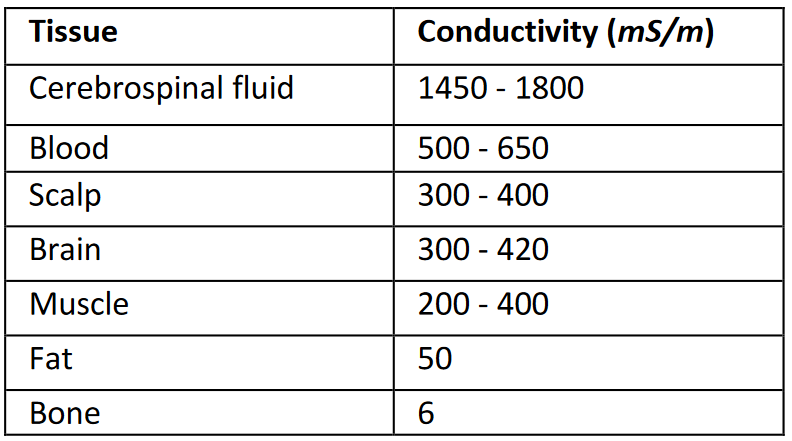
\includegraphics[width=3.05571in,height=1.70153in]{media/image2.png}~

The differences in conductivity are mapped out using electrical
excitation caused by two injection current sources. These two injection
currents have the same frequency and amplitude but are 180° out of phase
from each other. While one injection current is positively charged, the
other will be negatively charged. In conventional current terms, current
will flow from positive charge to negative charge. Electrodes
surrounding the tissue are used during the current injection process to
take voltage readings. Current injection sites are at the same locations
as the electrodes, but only 2 at a time are activated at once. The
turned-on current injectors rotate to the next injectors after a period
of time that is optimal for the measurement process. The current
injectors that are turned on depend on the process chosen. Figure (2)
shows a visualization of the injected currents streamlines traveling
between the two current injection sources.~

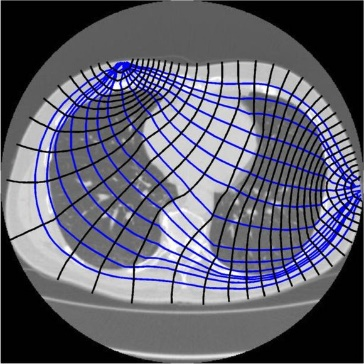
\includegraphics[width=1.64925in,height=1.64925in]{media/image3.jpeg}

~

\subsubsection{2.2.2 CLIENT BACKGROUND}\label{client-background}

Dr. Talles Santos received his Bachelor of Science degree in electrical
engineering from the federal University of Minas Gerais, Belo Horizonte,
Brazil, in 2012, Earned a master\textquotesingle s degree in 2015 and
his PhD in 2019, both in control engineering and mechanical automation
from the Polytechnic School at the University of São Paulo, Brazil.~~

Dr. Santos has more than 10 years of experience in the EIT field. He
worked part time at Timpel Medical, São Paulo, Brazil, working on EIT
development {[}3{]}. Also, he has worked with several other groups
developing EIT for medical applications. Currently he is a professor of
electrical engineering who is working for the University of Colorado,
Boulder. He now wants to start further development of EIT technology at
CMU, while using the opportunity to educate students in the principles
of how EIT works and how to construct a machine. Dr. Santos wants to
make the technology cheaper and more accessible to medical professionals
and individuals who want to study and help further develop the
technology {[}3{]}. EIT machines require the coordination of high
frequency current injection, sampling processes, and control circuitry
at high speeds in order to achieve real time imaging with a resolution
that is usable for a medical professional. The construction of such a
machine is a lot of work for one individual to undergo. The sponsor
requires the assistance of other individuals well versed in electrical
and computer engineering, which is the reason why the 2022-2023 capstone
team has been tasked with assisting the sponsor in the construction of
an EIT machine.

\subsubsection{CURRENT PROCESS}\label{current-process}

Currently there is no EIT machine working or in development at CMU. This
project will be the beginning of its development at CMU.

\subsubsection{EXISTING SOLUTIONS}\label{existing-solutions}

The existing solutions for this project are made by companies with
closed solutions. Some of the existing manufacturers are Timpel (Dr
Santos\textquotesingle{} former employer) {[}3{]}, Sentec {[}4{]},
Drager {[}5{]}, and Sciospec{[}6{]}. Sciospec replied to the team with a
quote for a medical grade 64 channel EIT machine the price is about
\$60k. This is outside the budget of the sponsor, and it severely limits
the modifications that can be made to the device. In addition, the
sponsor wants the project to be more open source and to not use
proprietary or expensive commercial hardware.

This means that this project will be building each component from the
ground up. The project sponsor has many years of experience in EIT
application and research. There are three major components to design.
First is a current injection system, second is the measurement system,
third is the control system.

First, the current injection system, which injects current into the
patient to be measured by the measurement system. There are specific
methods of current injection patterns, creating a stable current
injection source, and signal extraction that were recommended. For
current injection, the skip four method was recommended by our sponsor.
The skip four method is when the bipolar current injection is done
between two electrodes spaced 4 electrodes apart, at all times. There
are no current sources that would match our requirements and that would
be within our price range.

Second, the measurement system has three main requirements. First is the
precision of the system, second is the sampling frequency, and third is
synchronization of the measurements. The sponsor provided two National
Instruments PCI-6259 DAQ boards (NI boards for short) for the project.
These boards are 125 kS/s when using 32 channels that will have 1mV
precision with the ability to synchronize all the channels together.

Third, the control system, which oversees the current and measurement
systems so they can work together. This system needs to have the
processing power to run faster than the current and measurement systems
to be able to coordinate the systems together. There are many existing
solutions for the control system. Diego has proved an old desktop to
use. The desktop has the ability to connect the two measurement boards
to the motherboard and use the software to collect data and process it
into an image.

\subsection{DESIGN REQUIREMENTS/CRITERIA and Engineering Standards}
The project deliverable is a functioning EIT machine capable of:

\begin{itemize}
\item
  Three-Frequency Signal Generation

  \begin{itemize}
  \item
    Ideally consisting of 80, 100, and 120 kHz frequencies
  \item
    10mA RMS current injection

    \begin{itemize}
    \item
      Accurate within 0.1mA
    \end{itemize}
  \end{itemize}
\item
  32 Channels of voltage readings

  \begin{itemize}
  \item
    Sample size (500 - 1024)
  \item
    Use the two provided NI PCI-6259 DAQ boards (NI boards)

    \begin{itemize}
    \item
      Highest sampling rate possible with NI board
    \item
      Maximum rate of 1 MS/s single channel possible
    \end{itemize}
  \end{itemize}
\item
  Real-Time imaging

  \begin{itemize}
  \item
    Ideally 32x32 bits
  \end{itemize}
\item
  Buffer between measurement and electrodes
\item
  Control system to map the current delivery to desired electrodes

  \begin{itemize}
  \item
    Synchronizes with measurement process
  \item
    Implements the "skip 4 method"
  \end{itemize}
\item
  Safely limit current

  \begin{itemize}
  \item
    To ensure test subjects are not shocked
  \item
    To provide redundancy in power supply current protection
  \end{itemize}
\item
  Implement central control through the use of a desktop computer

  \begin{itemize}
  \item
    Use the computer monitor to display the real time imaging
  \end{itemize}
\item
  Develop a working process to rapidly prototype PCB boards
\item
  Use MATLAB to display imaging and process data
\end{itemize}

Three frequency current injection into the test subject is necessary for
various reasons due to the impedance characteristics of biological
tissue as described in section 4.2.1. Three frequency current injection
is favored as an optimal way that the sponsor has found to get a more
precise image. The 10 mA rms current amplitude is considered by the
sponsor to be sufficient to provide voltage readings that will be above
noise levels at a level that makes taking the voltage readings possible,
without injecting too much current that it becomes unsafe for a patient.
The skip four method of current injection has been shown through the
sponsor\textquotesingle s research to be the most effective way to
inject current for good imaging. The skip four method is when the two
current injection sources are spaced 4 electrodes away from each other,
and this pattern alternates in a clockwise pattern.

Thirty-two channels of voltage readings from the electrodes are
necessary to construct an image of the quality the sponsor is hoping to
achieve. Too low of a resolution on the image will leave the image
obtained from the device too difficult to be useful for medical
purposes. These 32 voltage readings are necessary to achieve a 32x32 bit
image. A minimum of 500 samples should be acquired in a buffer during
the sampling measurement process, with an ideal target 1024 samples.

Use of the NI boards provided is desired by the sponsor because it has
already existing toolboxes and has drivers available for simple
integration with MATLAB, which the sponsor desires for data processing
and imaging.

The desktop will be used for controlling the devices and for allowing
modular design as swapping in and out parts will be easier. The desktop
will be able to control the current injection source and the measurement
system at the same time to produce synchronized data. Then the desktop
will have the power to process the data into an image as the measurement
system takes another set of data to be processed. Implementing a
computer for central control in this way will simplify operation of the
EIT machine for the sponsor.

Published by the International Electrotechnical Commission (IEC), IEC
6061 is a list of technical standards for the safety and performance of
medical electrical equipment {[}7{]}. These standards are considered as
necessary in many countries by law and is widely accepted as a necessary
list of requirements for product development for many companies and
corporations. Another set of standards provided by the American National
Standard Institute is the ANSI/AAMI ES60601-1:2005, which also includes
standards on electrical equipment {[}8{]}. Standards that may apply to
the development of the EIT machine include calibration of the ADC and
electrical safety standards.

\section{Design Description}\label{design-description}

\subsection{OVERVIEW}\label{overview}

A computer with adequate clock speeds is critical to control multiple
running processes at the necessary speeds. A central computer will be
necessary to control and coordinate all the machine\textquotesingle s
components and processes. From this central control desktop computer,
two NI boards generate and read analog voltage signals and digital
signals. The generated analog voltage signals are used to control a
current source for injection into the test subject. The electrodes
receive the injection current directed by the control circuit,
controlled by the NI boards\textquotesingle{} digital output pins. While
the current injection is constantly occurring, the NI board reads all 16
electrodes placed around the test subject. These analog signals read
from the electrodes are then collected by a program and used to generate
a real-time image.

Coordinated by the control desktop using the NI Boards, a small
multifrequency signal is sent through a voltage controlled current
source. The signal is restricted to a consistent output despite the
body\textquotesingle s various impedances. Then the signal is directed
to the body\textquotesingle s active electrodes using the digital logic
from the desktop to the multiplexers. Using the same active electrodes,
the signal is both sent and read. The signal data is sent to the MATLAB
(software) script where the signal is properly extracted and
reconstructed into the image.

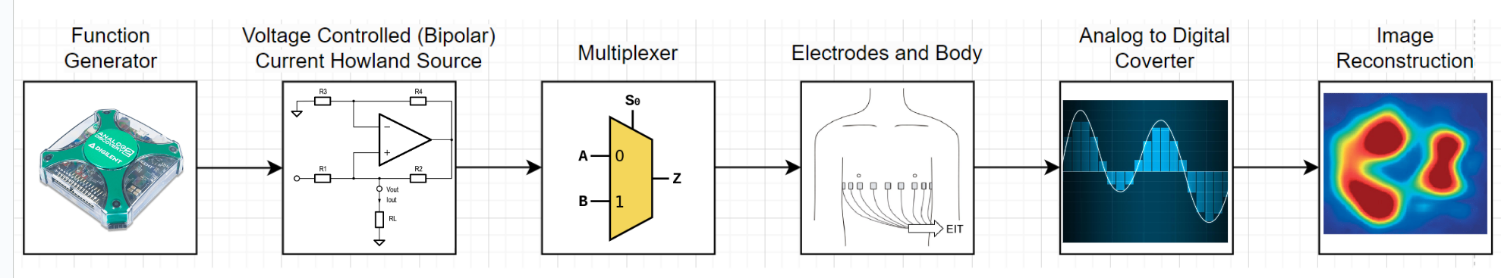
\includegraphics[width=6.83087in,height=1.26656in]{media/image4.png}

\subsection{DETAILED DESCRIPTION}\label{detailed-description}

\subsubsection{SYSTEM/COMPONENT 1 - Control}\label{systemcomponent-1---control}

The control system circuit consists of two 16:1 multiplexor (MUX) ICs.
The specific component used in the design was the ADG406BNZ, from Analog
Devices Inc. These MUXs are designed to direct 16 different signals to
or from one destination or source. The MUXs are being used to direct a
current from a respective Howland current source to one of 16
electrodes. The 16 MUX outputs connect the 16 electrodes with the NI
Boards read channels and are directed by 4 digital control signals.
Connecting each output of the MUXs will halve the amount of wire needed
and will not be an issue because the MUXs will not have the same
channels, permitting current flow at the same time. A single 12 V supply
will power the MUXs. A simple diagram of the control circuit is shown in
Figure 3.

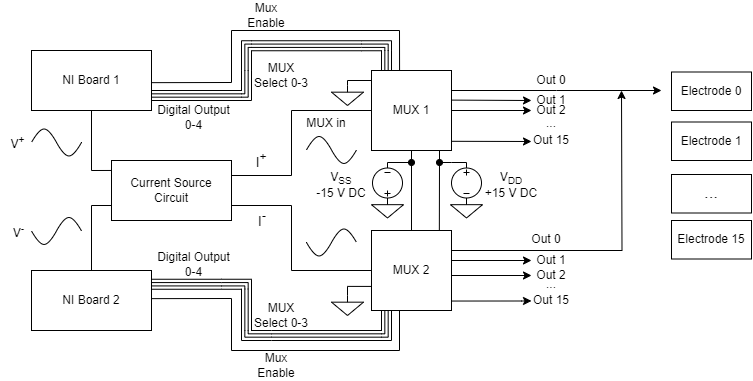
\includegraphics[width=6.5in,height=3.28889in]{media/image5.png}

\subsubsection{SYSTEM/COMPONENT 2 -- Current Injection}\label{systemcomponent-2-current-injection}

The current injection system consists of a multifrequency bipolar
signal. The signal contains a 10k, 25k, and 50k Hz signal with a peak
current of 10mA. The signals will be generated using the NI boards 180
degrees out of phase. The signal will then be sent through the Howland
current source where the current is restricted. The body has a varying
impedance as the patient breathes and the Howland current source keeps a
constant current output while impedance varies. Figure 4 below shows
both sides of a completed current source circuit.

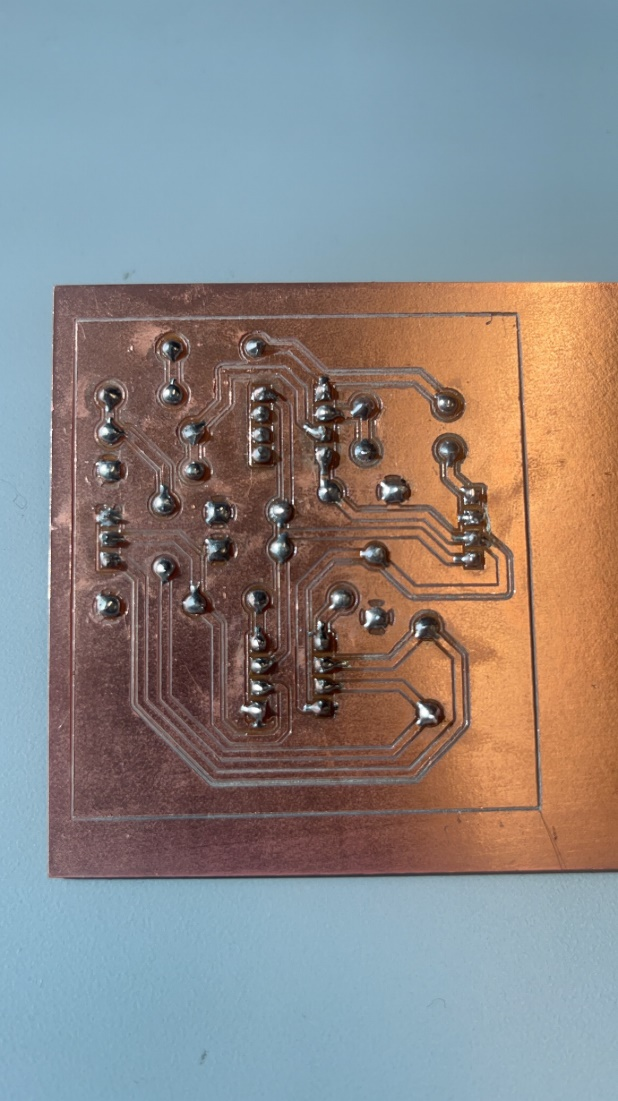
\includegraphics[width=2.56253in,height=2.30215in]{media/image6.jpeg}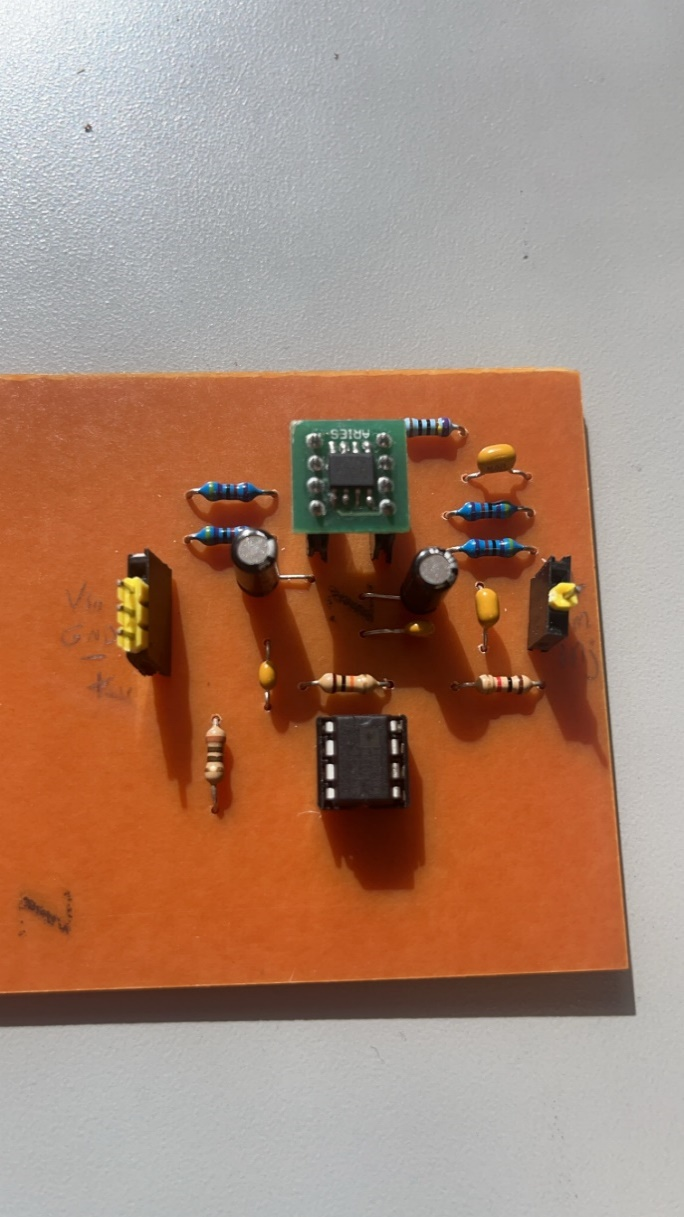
\includegraphics[width=2.6386in,height=2.29158in]{media/image7.jpeg}

\subsubsection{SYSTEM/COMPONENT 3 - Measurement}\label{systemcomponent-3---measurement}

The measurement system consists of 16 electrodes and two NI boards. The
NI boards read analog voltage signals from electrodes, which pick up
voltages created by the current injection system. The electrodes have
buffers that isolate the patient from the NI board and the current
directed by the MUX control circuit. The voltages read by the NI board
are then processed by a program written in MATLAB to create with code
supplied by Dr. Santos to create a real-time image. Figure 5 below shows
a simple layout of the active electrode circuit.

\includegraphics[width=6.5in,height=2.44167in]{media/image8.png}

\subsubsection{SYSTEM/COMPONENT 4 -- Power Supply}\label{systemcomponent-4-power-supply}


The power supply system provides power to all the IC components; each
requiring a different voltage. The first component running from a 60Hz,
120 V, standard AC wall outlet is a 120 V AC to 24 V DC converter.
Following this converter is multiple DC to DC converters. A 24 V DC to
plus and minus 15 V DC converter is used to provide power to the two
MUXs of the control circuit and provide power for the current source
circuit.

\subsection{USE}\label{use}

To be completed Later

\section{Evaluation}\label{evaluation}

\subsection{Overview}\label{overview-1}

The test plan for the EIT machine requires testing on many components.
To be confirmed was that two three-frequency voltage signals, consisting
of 10, 30, and 50 kHz, 180 degrees out of phase, were produced by the NI
board that was to be then converted into a current signal that was not
to exceed 10 mA, with a 1\% margin of error for accuracy. This current
signal delivery system was tested for accuracy and consistency with
voltage measurements by taking voltage measurements with an oscilloscope
over a resister.

A control system was also tested to ensure that timing and current
direction would be delivered to the appropriate electrodes at the
appropriate time. Testing of the control system was done by measuring
voltage signals at the electrodes while stepping through the control
system slowly while ensuring that the proper electrode was receiving the
signal. The control system was also to implement the skip-four pattern
of current injection.

The voltages produced on the electrodes were then to be read back in by
the ADC of the NI boards to processed by a MATLAB script. Ideally this
was to be done over 32 electrodes, at a sample rate of 1 Ms/s, verified
by settings designated by the created MATLAB script. At each each phase
of measurement, a single state of electrode current injection was to
provide a sample size between 500 to 1024 samples, which was simply
verified by viewing variables in MATLAB. MATLAB was also to be used to
provide real-time imaging, which would be verified by viewing a
real-time image of an object easily confirmed by placing objects in a
saltwater tank. A signal extraction technique was used to extract only
the desired input frequencies called Quadrature Demodulation and was
tested greatly to ensure its accuracy.

Current into the system used to power all circuitry needed to be current
limited as well to ensure safety. This was done by simply using
adjustable DC voltage sources using a single Gw Instek GPP-3323 DC power
supply. All circuits were to be done on CNC milled PCBs, was shown to be
completed with physically created PCBs that were implemented into use on
the EIT machine.

Table 4.1.1. Contains base requirements for EIT system.

\begin{itemize}
\item
  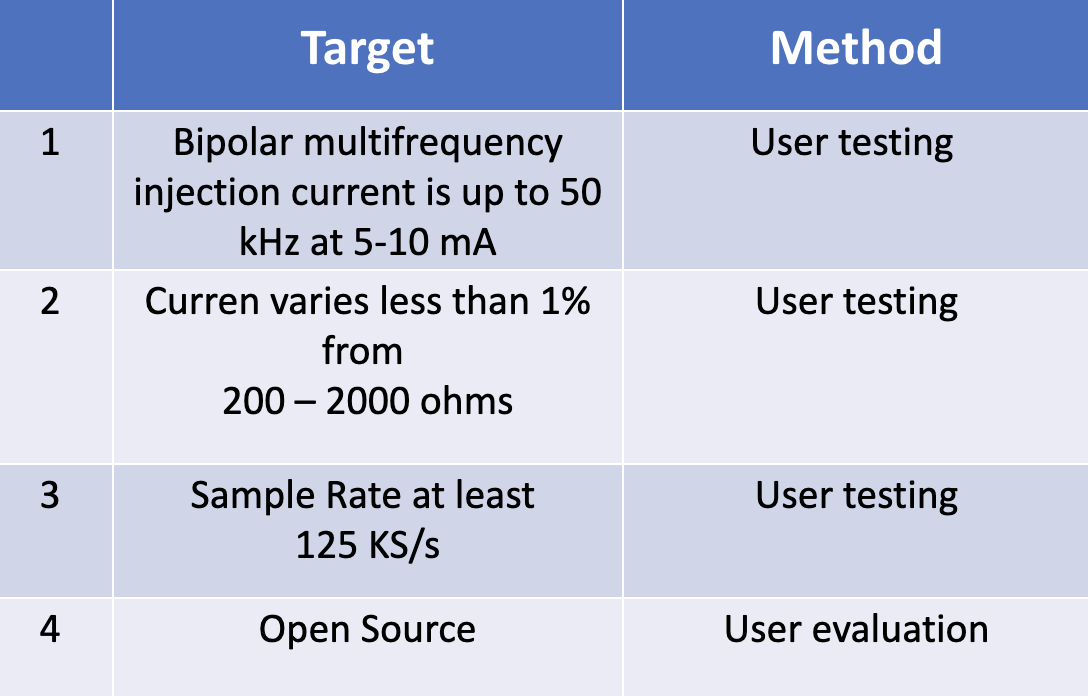
\includegraphics[width=4.59375in,height=2.94in]{media/image9.png}
\end{itemize}

\subsection{Evaluation of Howland Current Source Circuit and Signal Generation}\label{evaluation-of-howland-current-source-circuit-and-signal-generation}

\subsubsection{Purpose of Evaluation}\label{purpose-of-evaluation}

The signal sent to the patient must maintain a stable current across the
load resistance ranging from 500 to 2000 ohms. This requirement arises
from the fluctuating resistance within the patient\textquotesingle s
body, particularly during breathing cycles and lung inflation. It is
crucial to limit the deviation in current across these impedance ranges
to within 1\% to accurately capture the patient\textquotesingle s
impedance data, preventing distortion caused by signal artifacts. The
Howland current source employs DC-blocking capacitors at the signal
output to guarantee patient safety by preventing electric
shocks.\phantomsection\label{_Toc624427094}{}

\subsubsection{4.2.2 Test Methods}}\label{test-methods}

A single Howland circuit was tested with a variation of loads with an
input signal at the maximum frequency of 50kHz and a 6Vpp signal. This
expected approximately 7.75 mA output at 50kHz. This test allows the
current to be as high as possible without beginning to saturate.

\subsubsection{4.2.3 Results and Discussion}\label{results-and-discussion}

When the current surpasses 8mA at 1500 ohms, the output signal begins to
saturate due to the operational constraints of the Howlands AD8066 IC,
which is powered by +/- 12 volts and cannot exceed this output value. To
accommodate a resistance load of up to 2000 ohms, the design is limited
to utilizing up to 6 mA. Considering the system will be tested on a tank
with a resistance load of no more than 1500 Ohms, a current of 7.75 mA
is applied to optimize performance while avoiding saturation, as
indicated in Table 2. The table also displays an injection current error
within 6.4\%. Despite this proximity to the expected accuracy, it falls
short of the desired 1\% threshold set by our sponsor. Consequently, the
generated images may exhibit minor distortion if impedance fluctuates
between the minimum and maximum values.

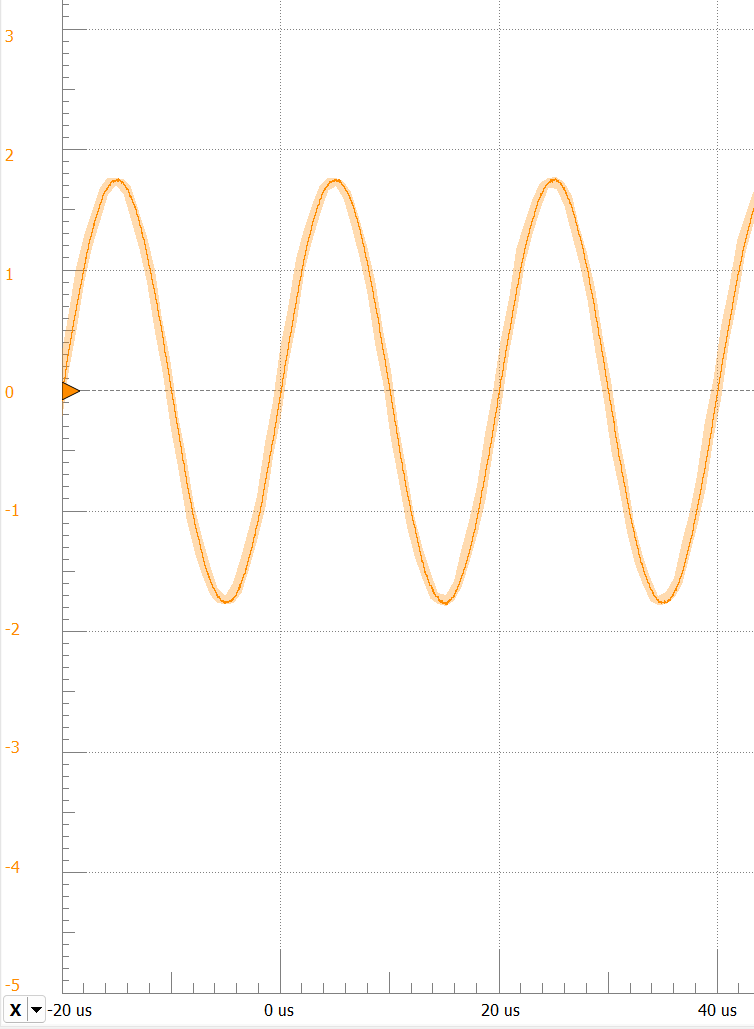
\includegraphics[width=4.61435in,height=4.23958in]{media/image10.png}

\begin{longtable}[]{@{}
  >{\raggedright\arraybackslash}p{(\columnwidth - 8\tabcolsep) * \real{0.2294}}
  >{\raggedright\arraybackslash}p{(\columnwidth - 8\tabcolsep) * \real{0.2504}}
  >{\raggedright\arraybackslash}p{(\columnwidth - 8\tabcolsep) * \real{0.1826}}
  >{\raggedright\arraybackslash}p{(\columnwidth - 8\tabcolsep) * \real{0.0824}}
  >{\raggedright\arraybackslash}p{(\columnwidth - 8\tabcolsep) * \real{0.2553}}@{}}
\caption{Table 1: Shows the difference in conductivity between different
tissue types~{[}1{]}}\tabularnewline
\toprule\noalign{}
\begin{minipage}[b]{\linewidth}\raggedright
Voltage Drop (Vpp)
\end{minipage} & \begin{minipage}[b]{\linewidth}\raggedright
Load Resistance (ohm)
\end{minipage} & \begin{minipage}[b]{\linewidth}\raggedright
Current (mA)
\end{minipage} & \begin{minipage}[b]{\linewidth}\raggedright
\end{minipage} & \begin{minipage}[b]{\linewidth}\raggedright
Current Difference (µA)
\end{minipage} \\
\midrule\noalign{}
\endfirsthead
\toprule\noalign{}
\begin{minipage}[b]{\linewidth}\raggedright
Voltage Drop (Vpp)
\end{minipage} & \begin{minipage}[b]{\linewidth}\raggedright
Load Resistance (ohm)
\end{minipage} & \begin{minipage}[b]{\linewidth}\raggedright
Current (mA)
\end{minipage} & \begin{minipage}[b]{\linewidth}\raggedright
\end{minipage} & \begin{minipage}[b]{\linewidth}\raggedright
Current Difference (µA)
\end{minipage} \\
\midrule\noalign{}
\endhead
\bottomrule\noalign{}
\endlastfoot
7.61 & 999 & 7.61 & & 510 \\
3.71 & 468 & 7.93 & & \\
11.06 & 1490 & 7.42 & & Percent Error (\%) \\
& & & & 6.4 \\
\end{longtable}

\subsection*{4.3 Evaluation of Quadrature
Demodulation}\label{evaluation-of-quadrature-demodulation}
\addcontentsline{toc}{subsection}{4.3 Evaluation of Quadrature
Demodulation}

\subsubsection*{\texorpdfstring{\textbf{4.3.1 Purpose of
Evaluation}}{4.3.1 Purpose of Evaluation}}\label{purpose-of-evaluation-1}
\addcontentsline{toc}{subsubsection}{\textbf{4.3.1 Purpose of
Evaluation}}

Quadrature demodulation (QD) is a technique that uses matrix math to
extract only a desired frequency from a signal that likely has
significant noise. This method in its application to data processing of
voltage signals gathered during the operation of the EIT machine was to
extract the amplitude, phase, and DC offset of a signal, figure which
would then be used to produce an image of relatively varying impedance.
The QD was tested by comparing the extracted signal to the original
signal to find the percent error difference.

\subsubsection*{\texorpdfstring{\textbf{4.3.2 Test
Methods}}{4.3.2 Test Methods}}\label{test-methods-1}
\addcontentsline{toc}{subsubsection}{\textbf{4.3.2 Test Methods}}

A three-frequency signal was generated with white noise added in using
MATLAB. A digital voltage was generated in MATLAB and saved then used to
produce a voltage on DAC pins of the NI board. Voltage readings were
taken using the ADC pins of the NI board. Then quadrature demodulation
was applied to measured voltages and processed using a MATLAB script to
extract the original individual 3 frequencies that made up the signal.
The signals read were then compared to the saved array of the originally
generated signal and compared. The percentage error was calculated
between the two signals.

\subsubsection*{\texorpdfstring{\textbf{4.3.3 Results and
Discussion~}}{4.3.3 Results and Discussion~}}\label{results-and-discussion-1}
\addcontentsline{toc}{subsubsection}{\textbf{4.3.3 Results and
Discussion~}}

The results from the testing are that the within 2\% of the original
amplitude and have 100\% of the original phase from each frequency. The
next test would be using the Howland currant source and MUXs to direct
the signal into the NI boards to measure the signal. Then quadrature
demodulation was then used to confirm the amplitude and phase of the
signal. Figure 7 is the three-frequency signal made of 10, 30, 50 kHz
sine waves without random noise, figure 8 is the same signal with 3dB of
random noise. Then figure 9-11 is the individual frequency demodulation,
showing the amplitude of each component frequency. Finally, figure 12 is
the summed components of the frequency demodulation to remove the noise
from the signal so it can be compared with figure 7.

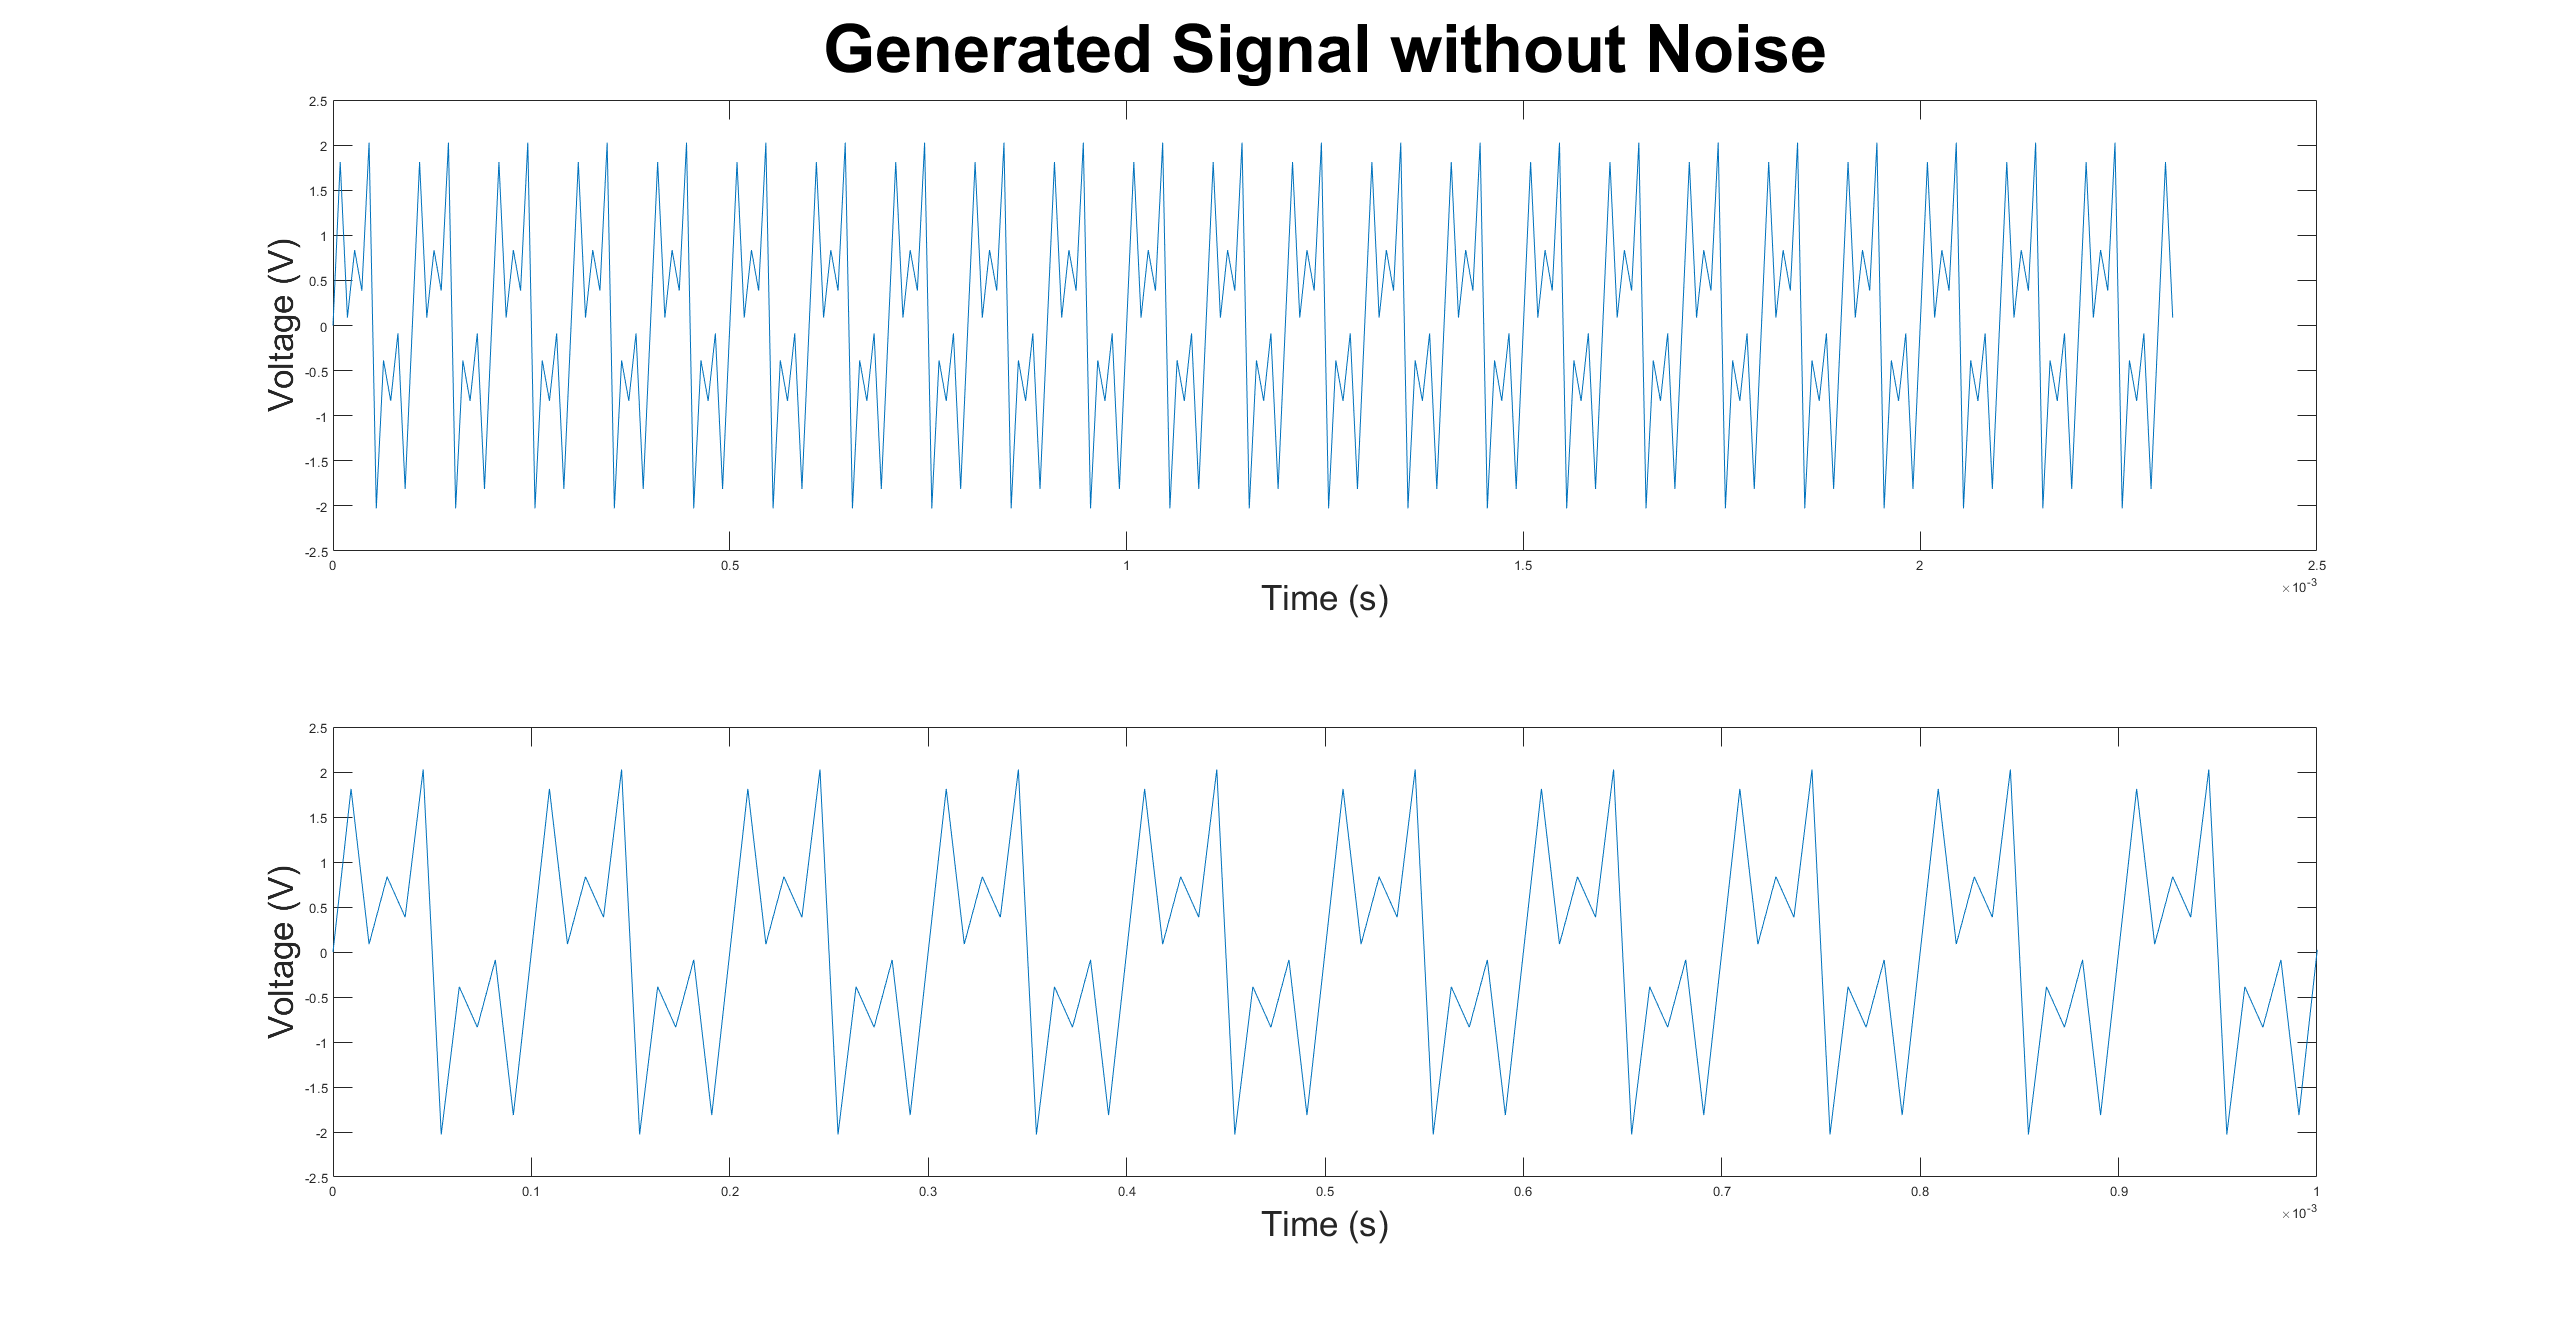
\includegraphics[width=6.5in,height=3.35903in]{media/image11.png}

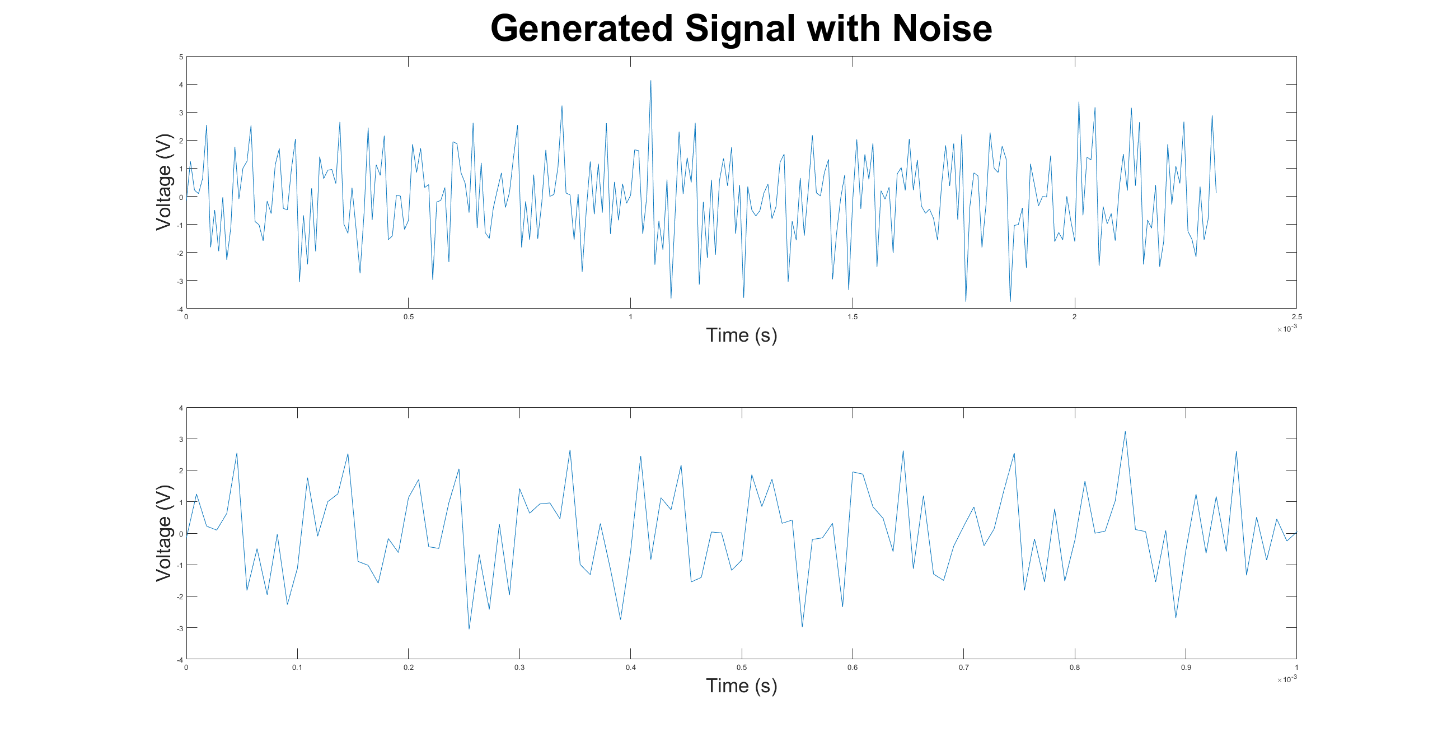
\includegraphics[width=6.47861in,height=3.34813in]{media/image12.png}

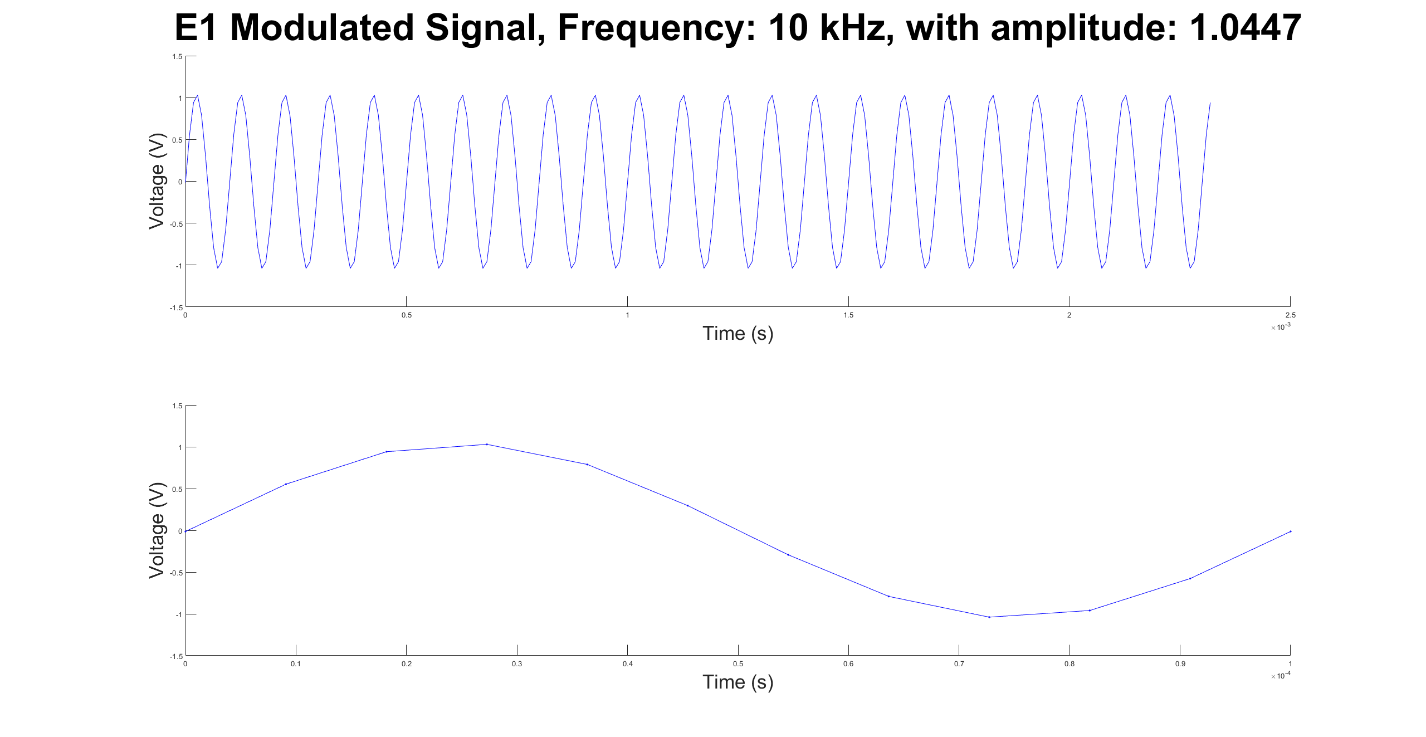
\includegraphics[width=6.47847in,height=3.34805in]{media/image13.png}

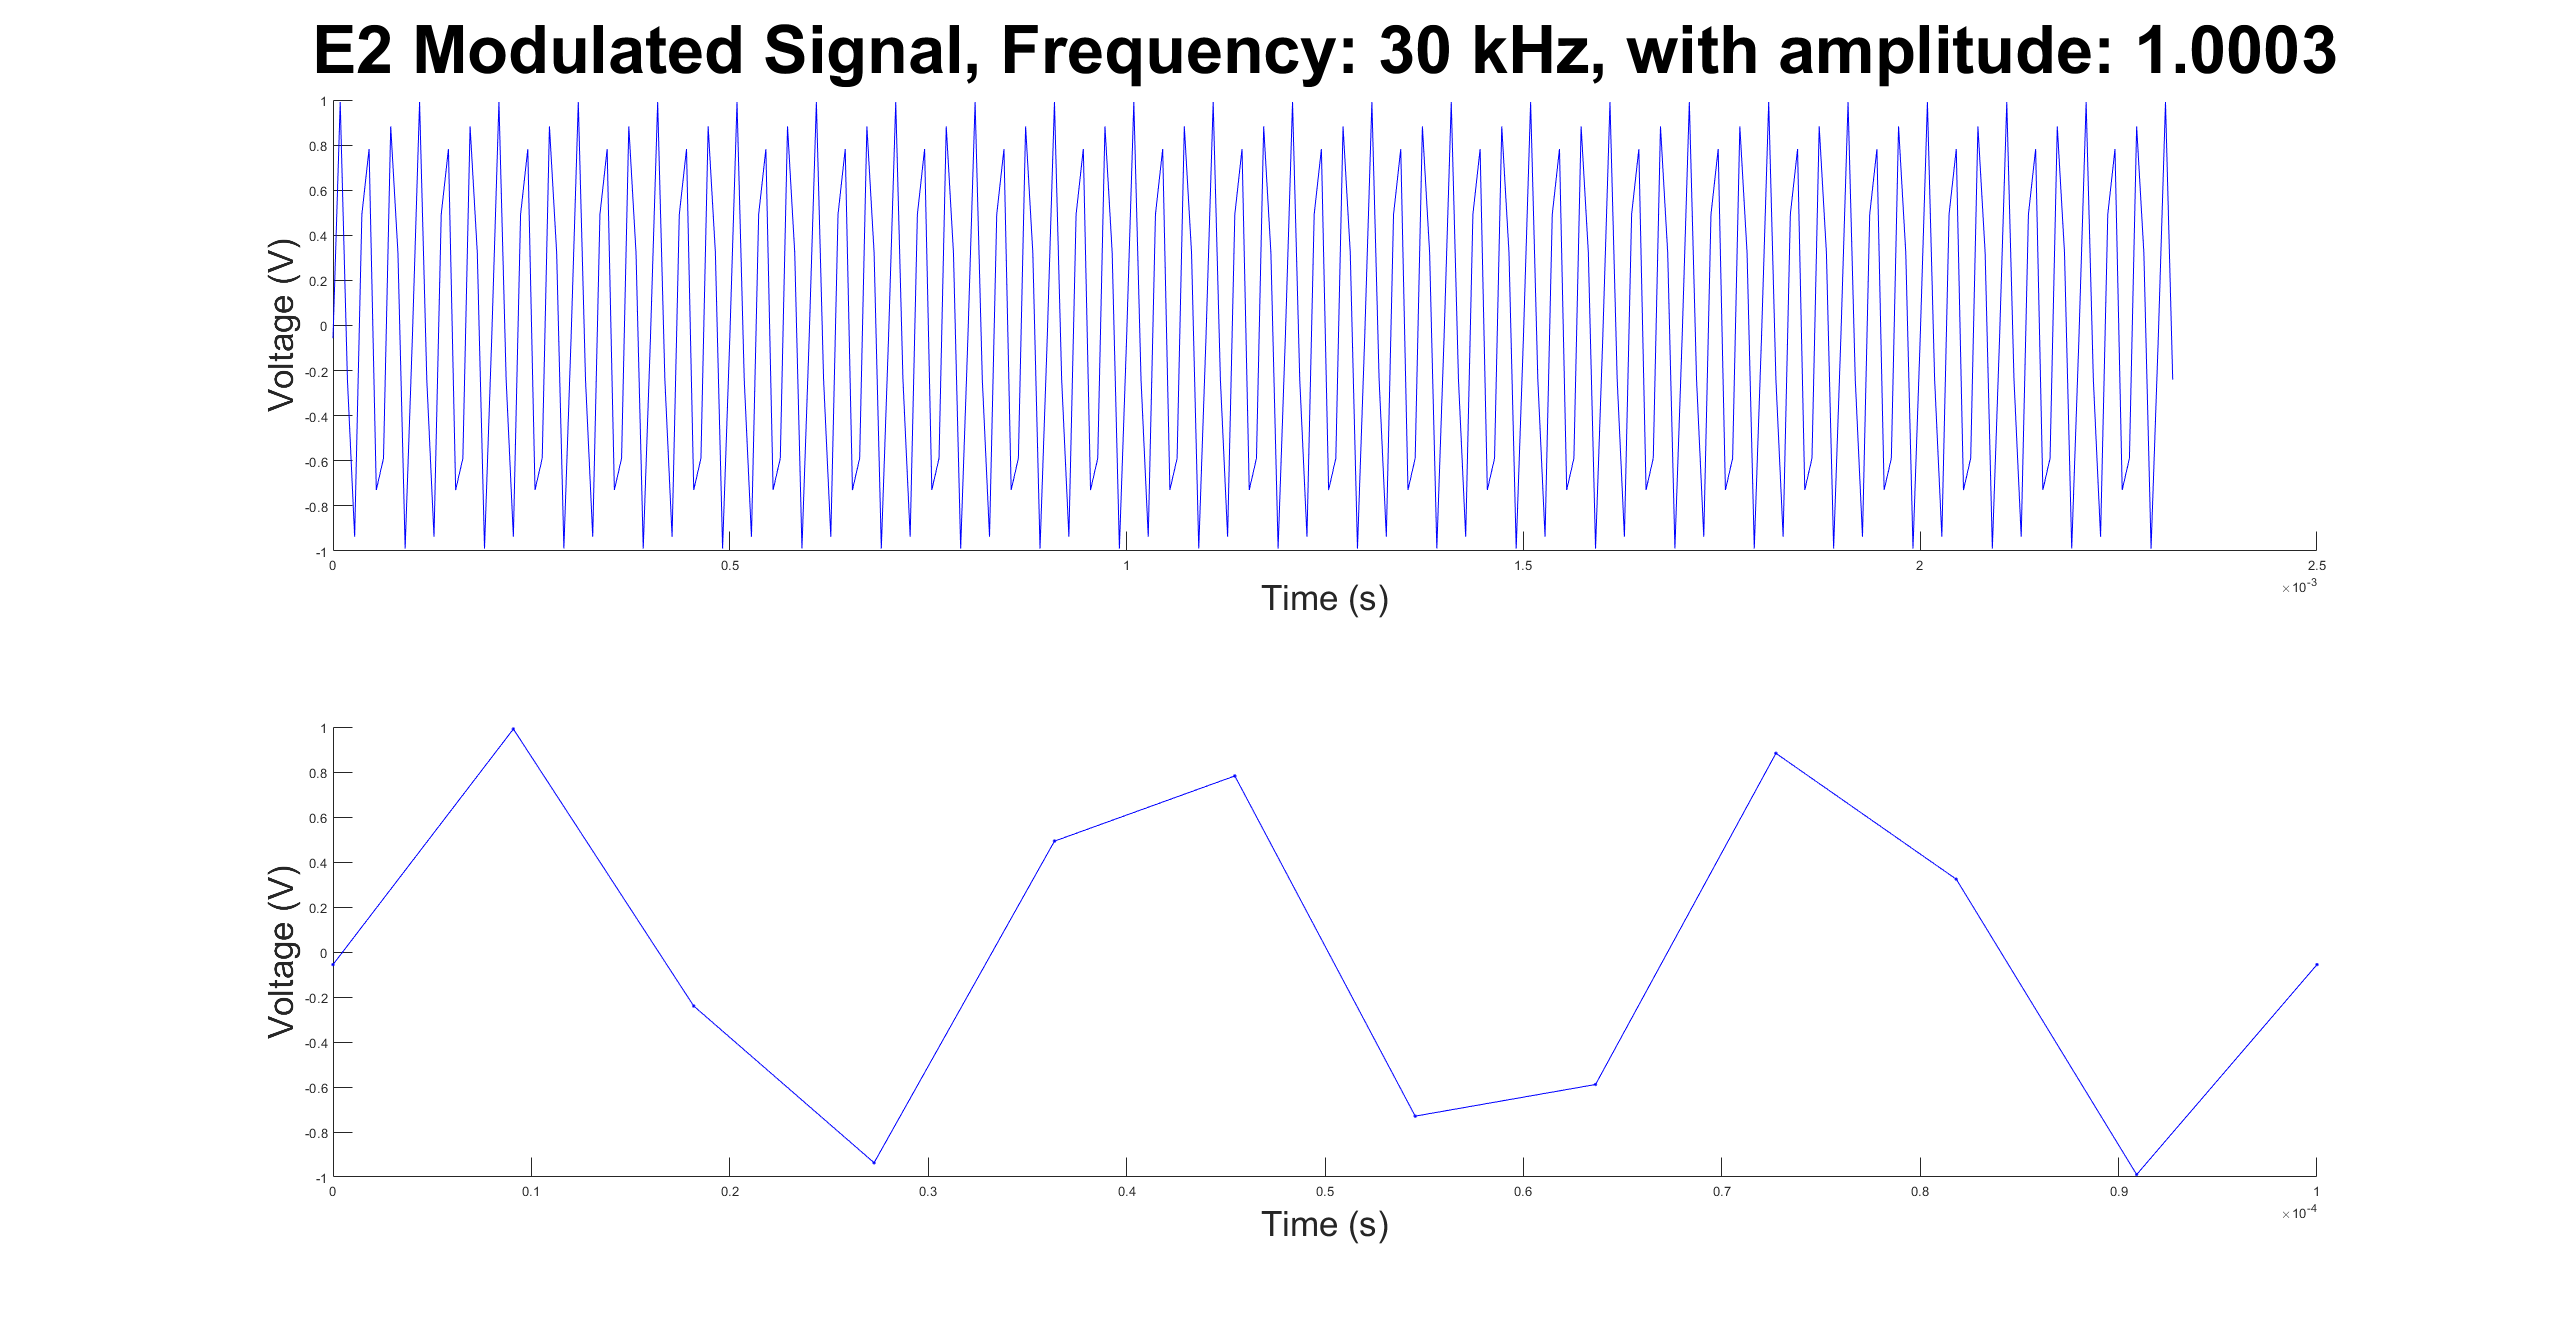
\includegraphics[width=6.47861in,height=3.34813in]{media/image14.png}

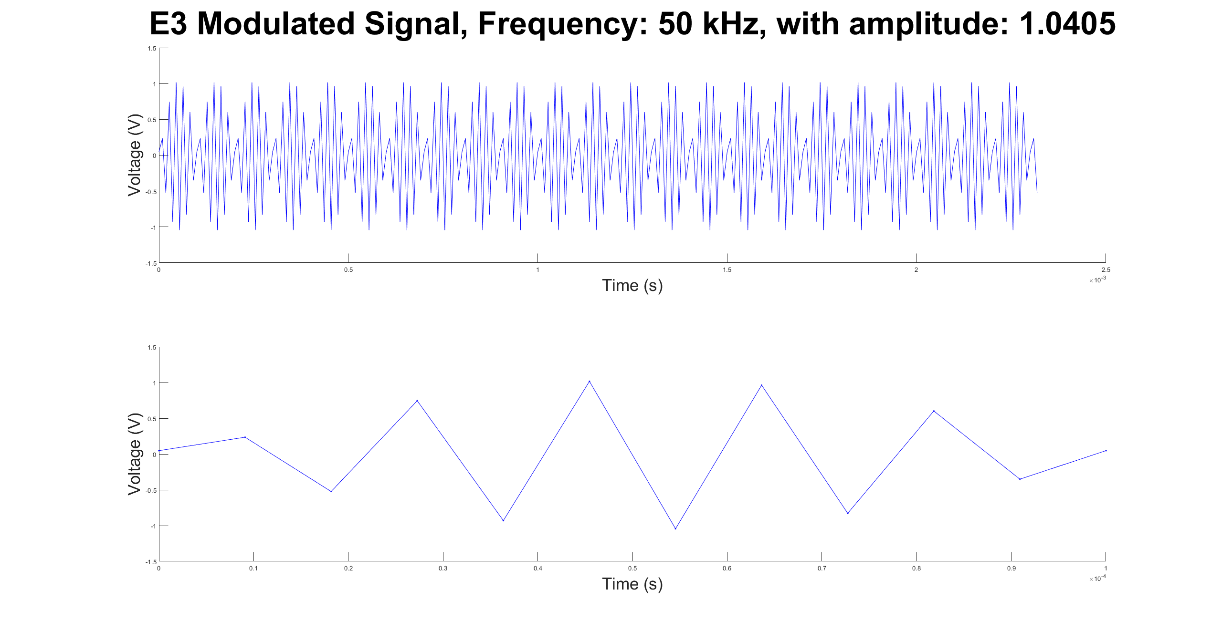
\includegraphics[width=6.47861in,height=3.34813in]{media/image15.png}

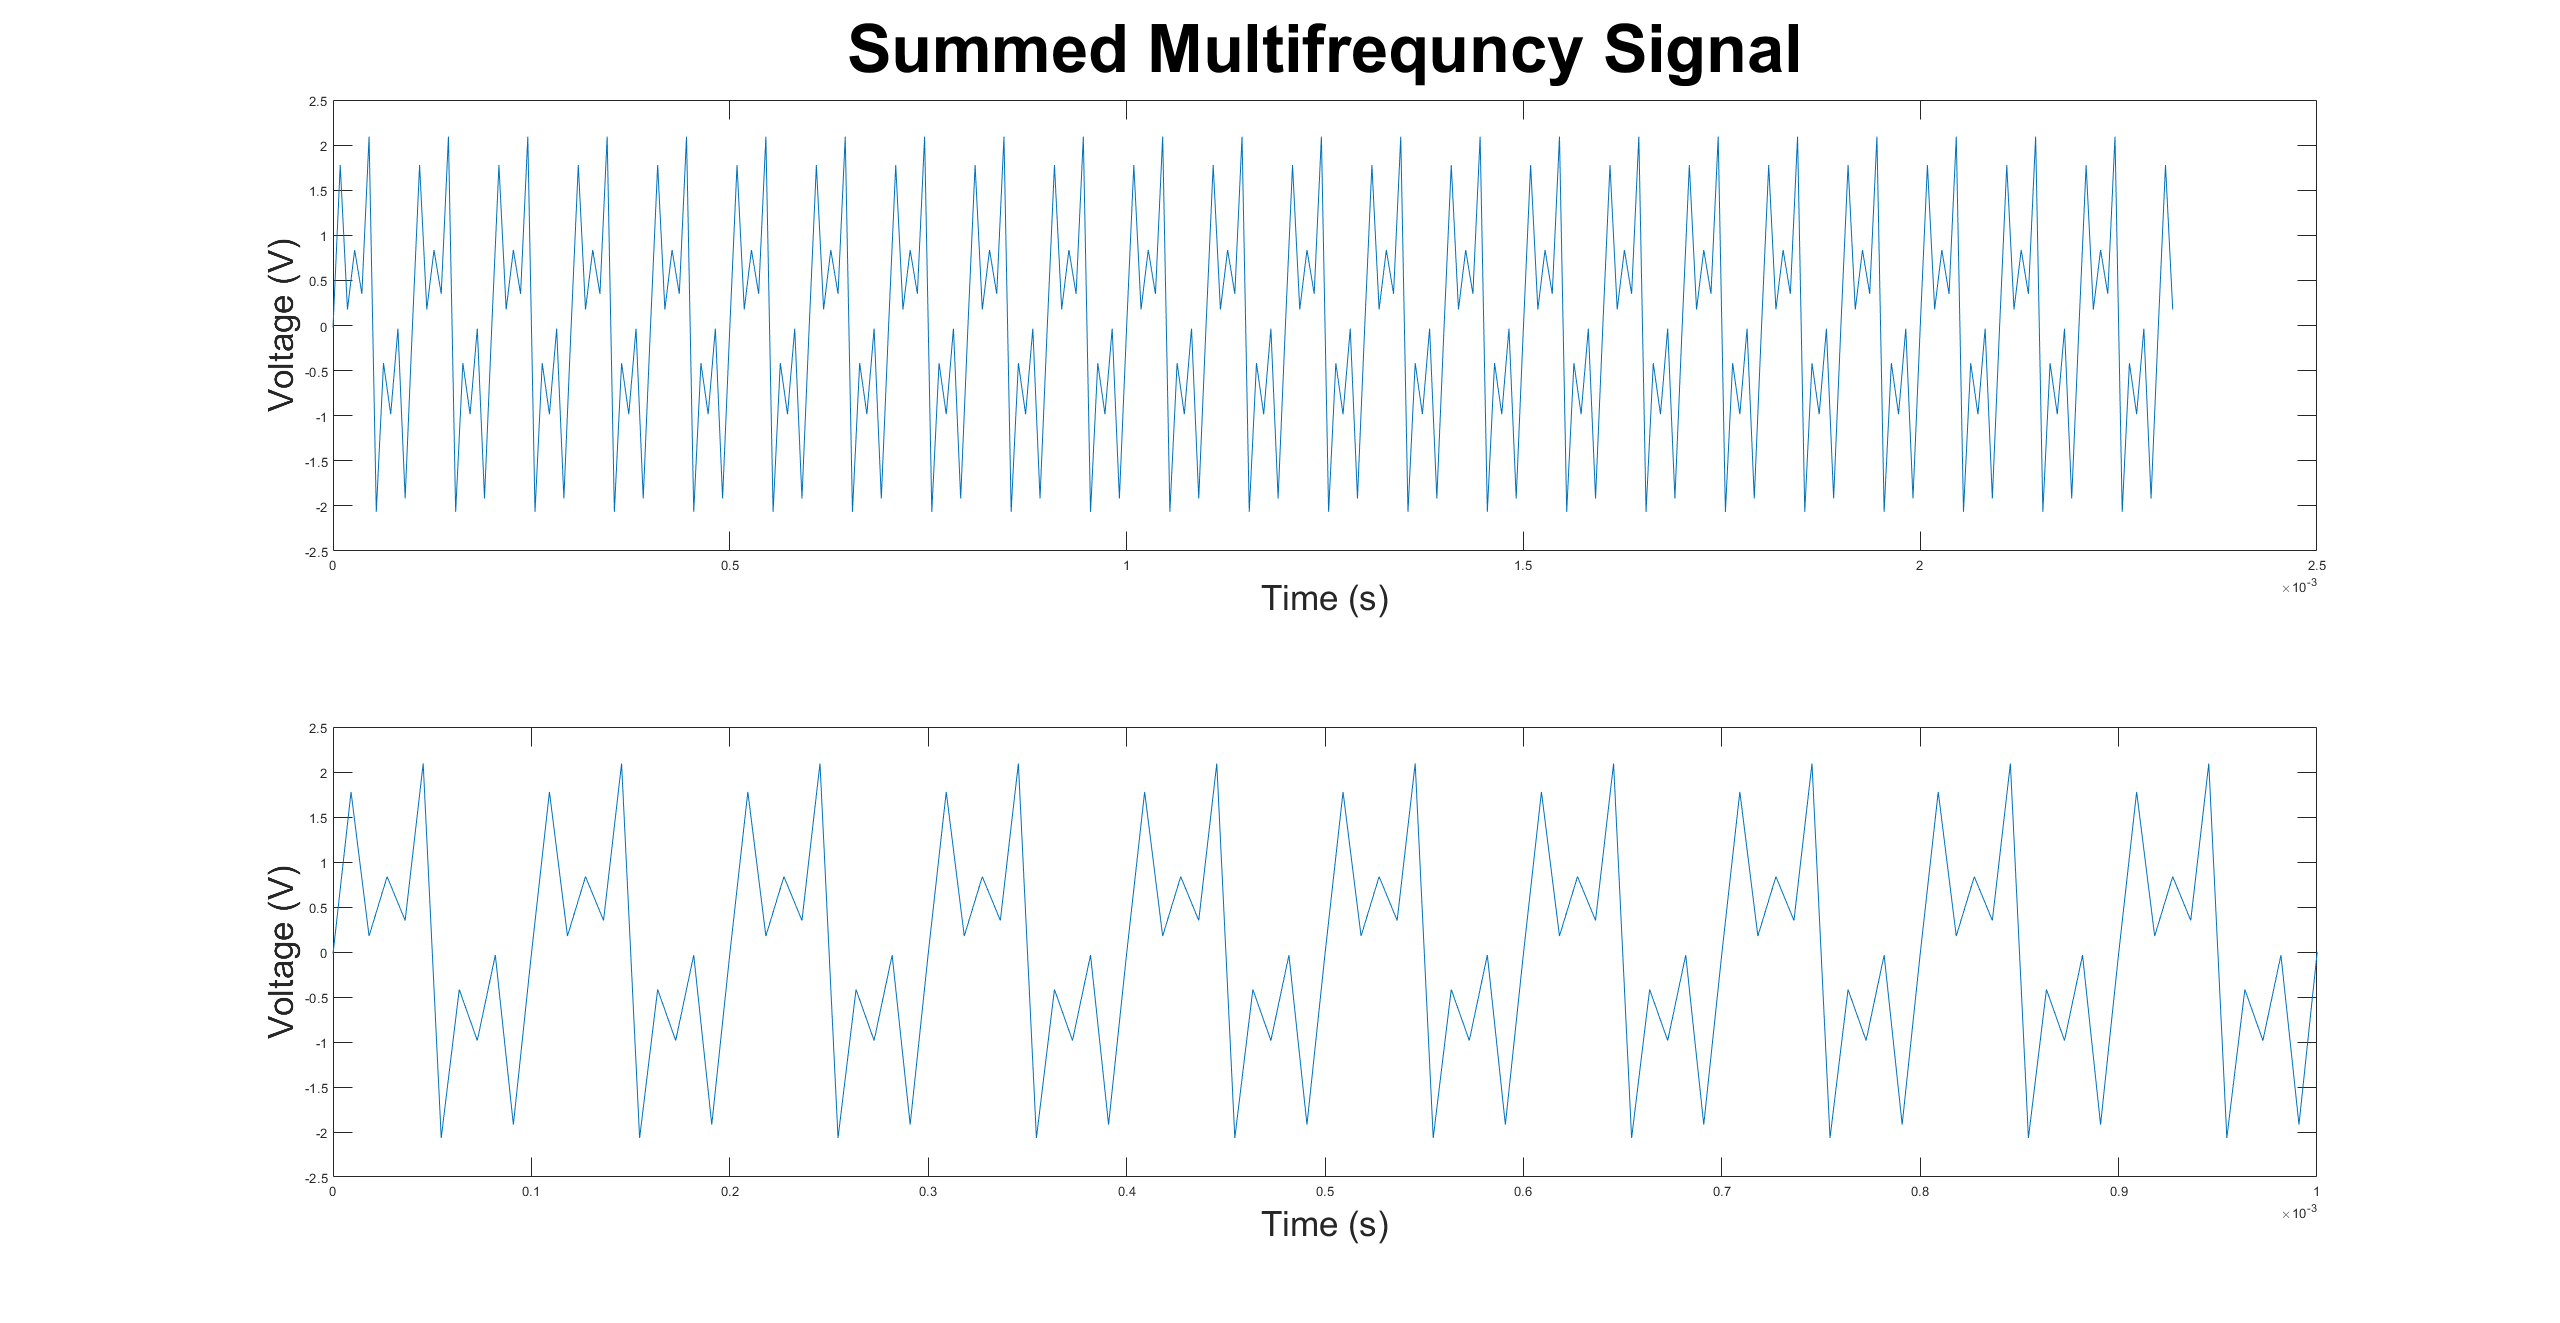
\includegraphics[width=6.47861in,height=3.34797in]{media/image16.png}

\subsection*{4.4 Evaluation of Control
System}\label{evaluation-of-control-system}
\addcontentsline{toc}{subsection}{4.4 Evaluation of Control System}

\subsubsection*{\texorpdfstring{\textbf{4.4.1 Purpose of
Evaluation}~}{4.4.1 Purpose of Evaluation~}}\label{purpose-of-evaluation-2}
\addcontentsline{toc}{subsubsection}{\textbf{4.4.1 Purpose of
Evaluation}~}

The purpose of the central control system is to direct all circuits and
signals with a desktop computer and MATLAB. The system used the NI PCI
boards for analog and digital outputs to control the Howland current
source, mux current direction, electrode current selection. The criteria
that the control system needed to meet were simple; direct current flow
to appropriate electrodes. The pattern followed was one where the two
bipolar currents are to be spaced apart by four electrodes in a
16-electrode set up, at all times, in a clockwise pattern and was
verified by oscilloscope voltage measurements.

\subsubsection*{\texorpdfstring{\textbf{4.4.2 Test Methods}
}{4.4.2 Test Methods }}\label{test-methods-2}
\addcontentsline{toc}{subsubsection}{\textbf{4.4.2 Test Methods} }

The first test that took place was to ensure the MUX control circuit
could be controlled properly by the MATLAB script and NI board.
Verification of the MUX control circuit was done by wiring the select
bit pins to digital output pins of the NI board and ensuring that an
output signal could be directed to the output from one of the 16 input
channels desired.

After verification that the MUX control circuit functioned properly, the
electrodes were wired to the outputs of the MUX control circuit. The
Electrodes required switches to be digitally controlled by digital
output pins on the NI board. The MATLAB script was modified to time the
output electrode switches to connect to the outputs of the MUX circuit.
The script was then stepped through to ensure that the MATLAB script was
properly controlling the digital outputs to direct the current flow to
the proper electrodes. This testing was done in phases of testing 4
electrodes, then 8, and finally 16. Testing was done over resistors as
well as over a saltwater tank created for testing, which is shown in
Figure 4.4.2.1, below.

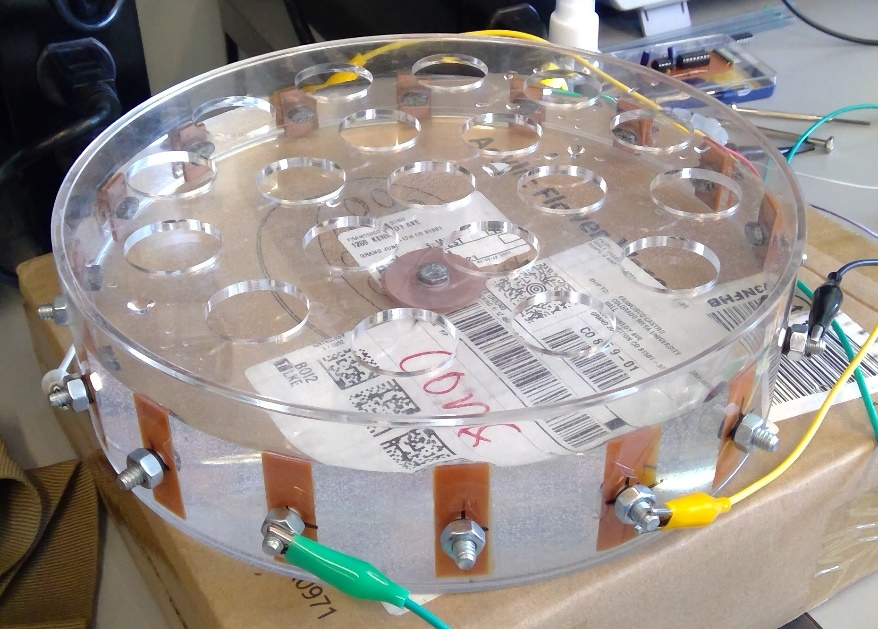
\includegraphics[width=3.98457in,height=2.85416in]{media/image17.jpeg}

Figure 4.4.2.1: Example of test set up for salt water testing tank

\subsubsection*{\texorpdfstring{\textbf{4.4.3 Results and
Discussion}~}{4.4.3 Results and Discussion~}}\label{results-and-discussion-2}
\addcontentsline{toc}{subsubsection}{\textbf{4.4.3 Results and
Discussion}~}

Results of testing electrode measurements over resistors and the testing
tank are shown below. Figures 4.4.3.1 and 4.4.3.2 show testing of
voltage readings over the saltwater testing tank using 4 electrodes,
using a skip 0 pattern. Figure one shows voltage readings without a
ground connected electrode, which was built into the center bottom of
the tank. Figure 4.4.3.2 shows the same setup but with the grounding
electrode connected to circuit ground. To note is the fact that in
Figure 4.4.3.1, the Measured Raw Data plot does not show the two
injection currents, which are of the greatest amplitude, 180 degrees out
of phase as they should be. However, Figure 2 shows the two greatest
amplitude signals of the raw data as properly 180 degrees out of phase.
In the Current Raw Data of both Figures 4.4.3.1 and 4.4.3.2, the
amplitudes of current do not match in amplitude as they should. Figure
4.4.3.1 Raw Data Measurements does show voltage readings that are
expected, however there is a slight issue in a difference of amplitude
that can be seen in the two greatest amplitude sine waves.

Figures 4.4.3.3 and 4.4.3.4 are voltage measurements using an
8-electrode system over resistors instead of the saltwater testing tank.
Measurements present the same characteristics noticed in the 4
electrodes system. The main difference would be that in Figure 4.4.3.3,
the measurements with a 100 kilo-Ohm in parallel with the 1 kilo-Ohm
resistors connecting the electrodes to ground has a significantly
smaller voltage, as would be expected, for the electrodes not with an
active injection current.

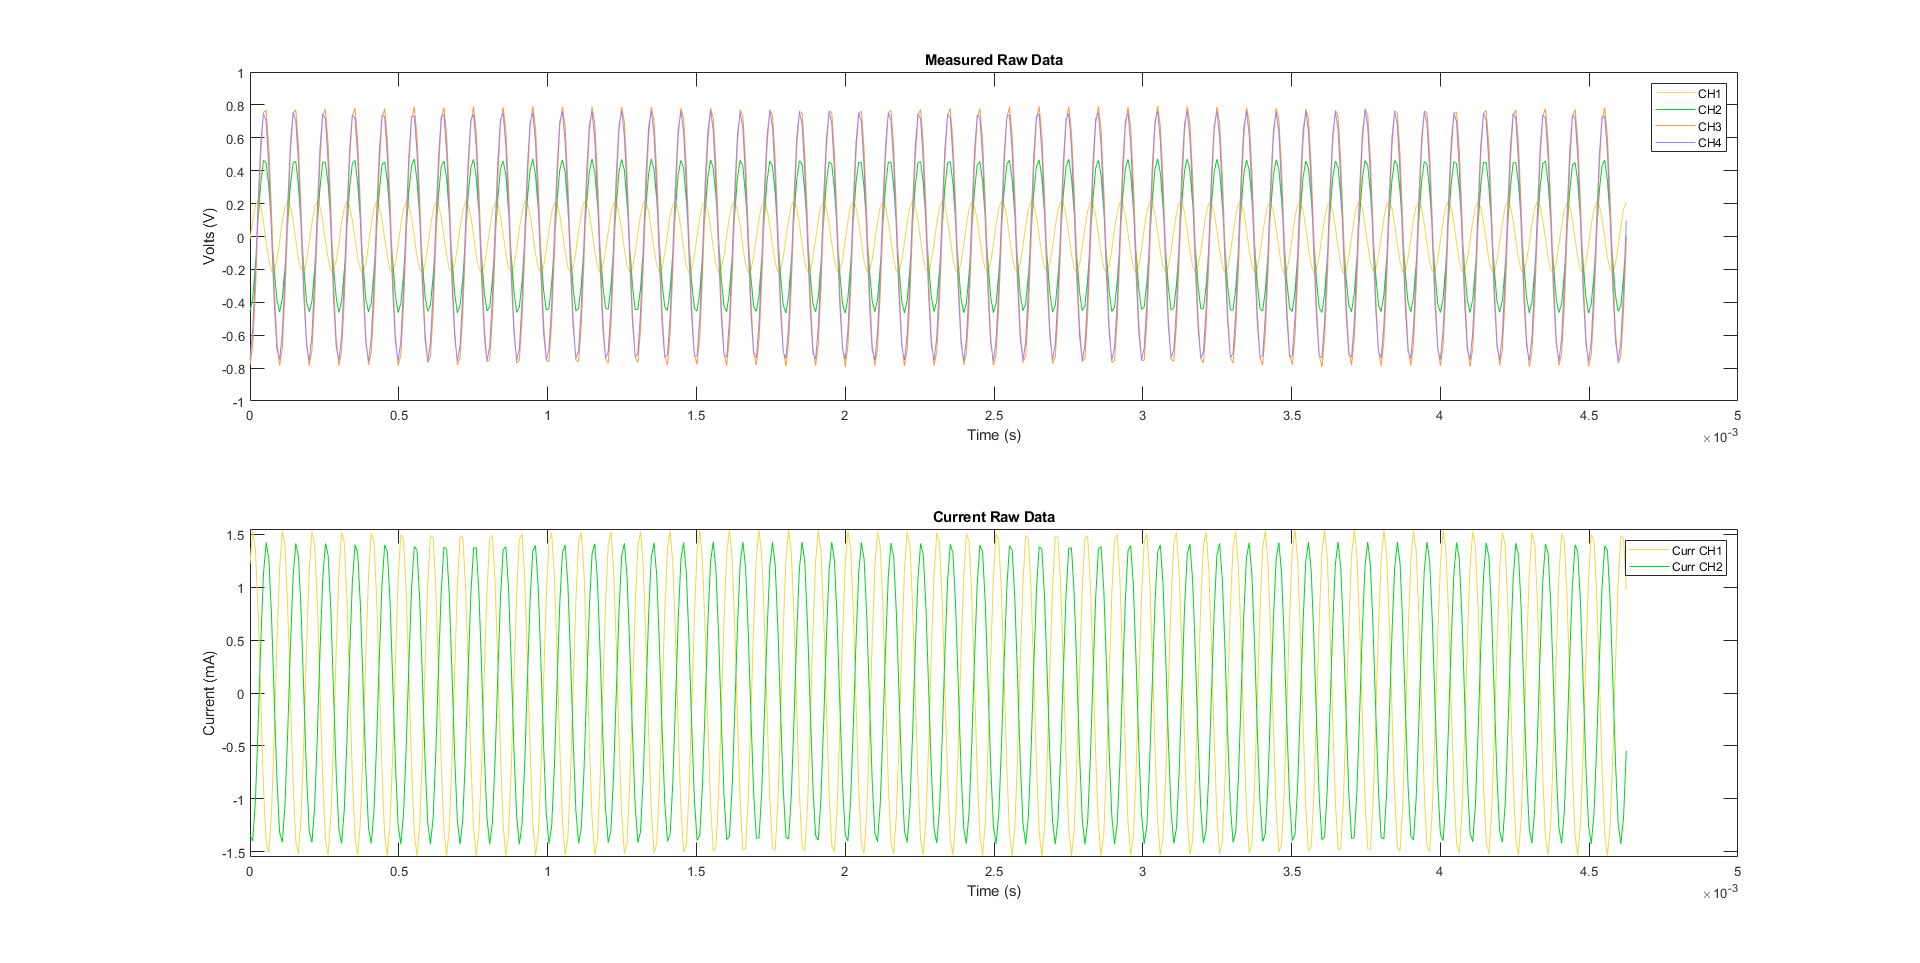
\includegraphics[width=6.5in,height=3.26181in]{media/image18.png}

Figure 4.4.3.1: Test showing voltage readings from 4 electrodes without
a ground on the tank with skip zero pattern

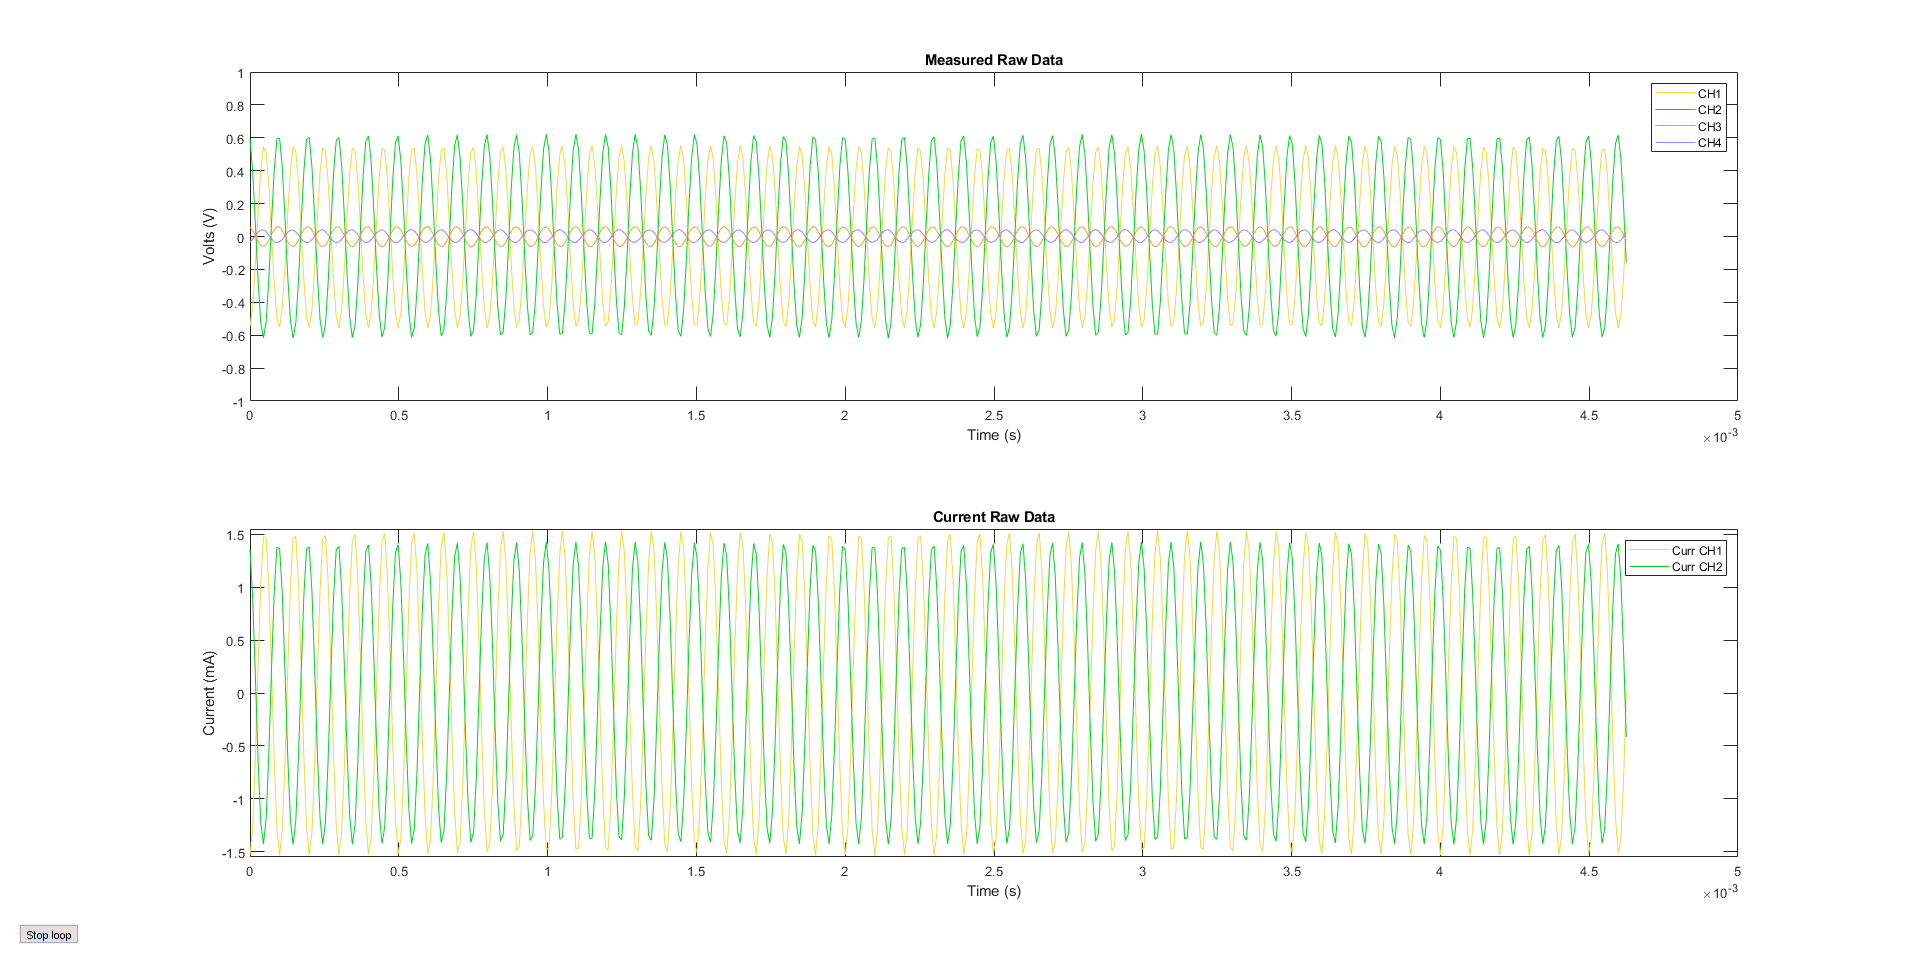
\includegraphics[width=6.5in,height=3.26181in]{media/image19.png}

Figure 4.4.3.2: Test showing voltage readings from 4 electrodes with a
ground on the tank with skip zero pattern

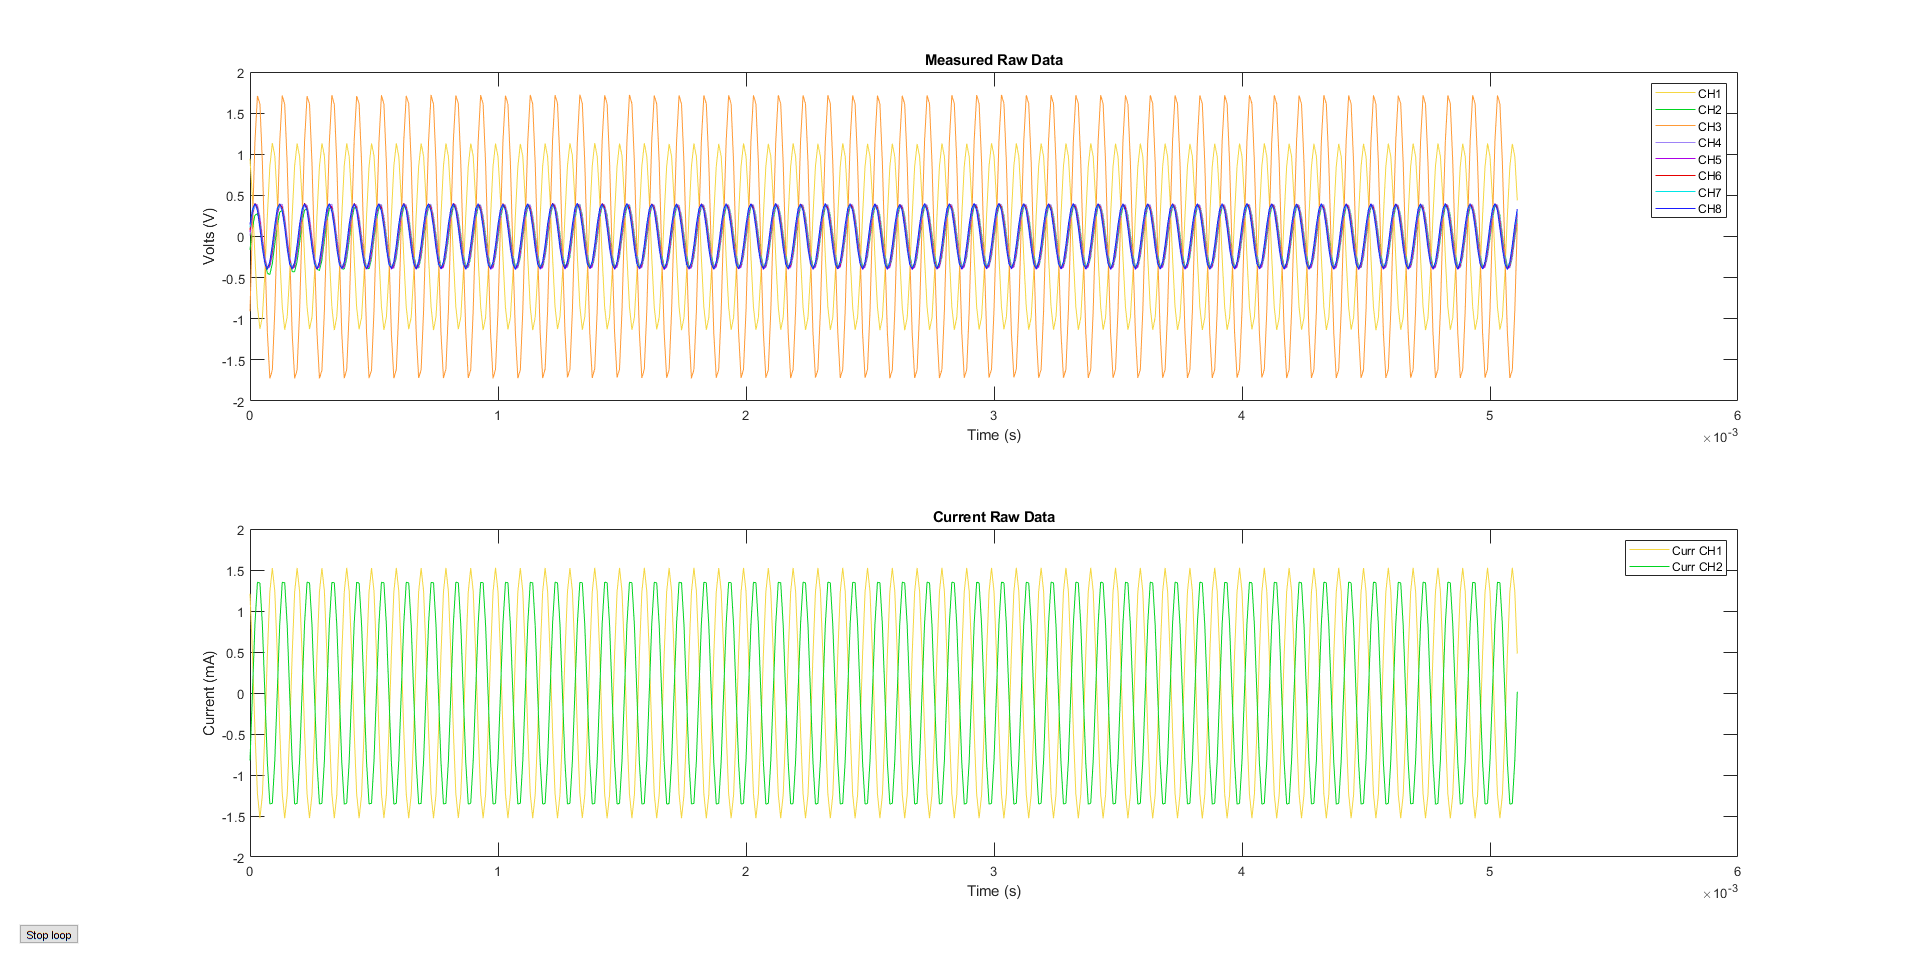
\includegraphics[width=6.5in,height=3.26181in]{media/image20.png}

Figure 4.4.3.3: Shows a plot of the voltage readings while testing 8
electrode channels over resistors instead of the
tank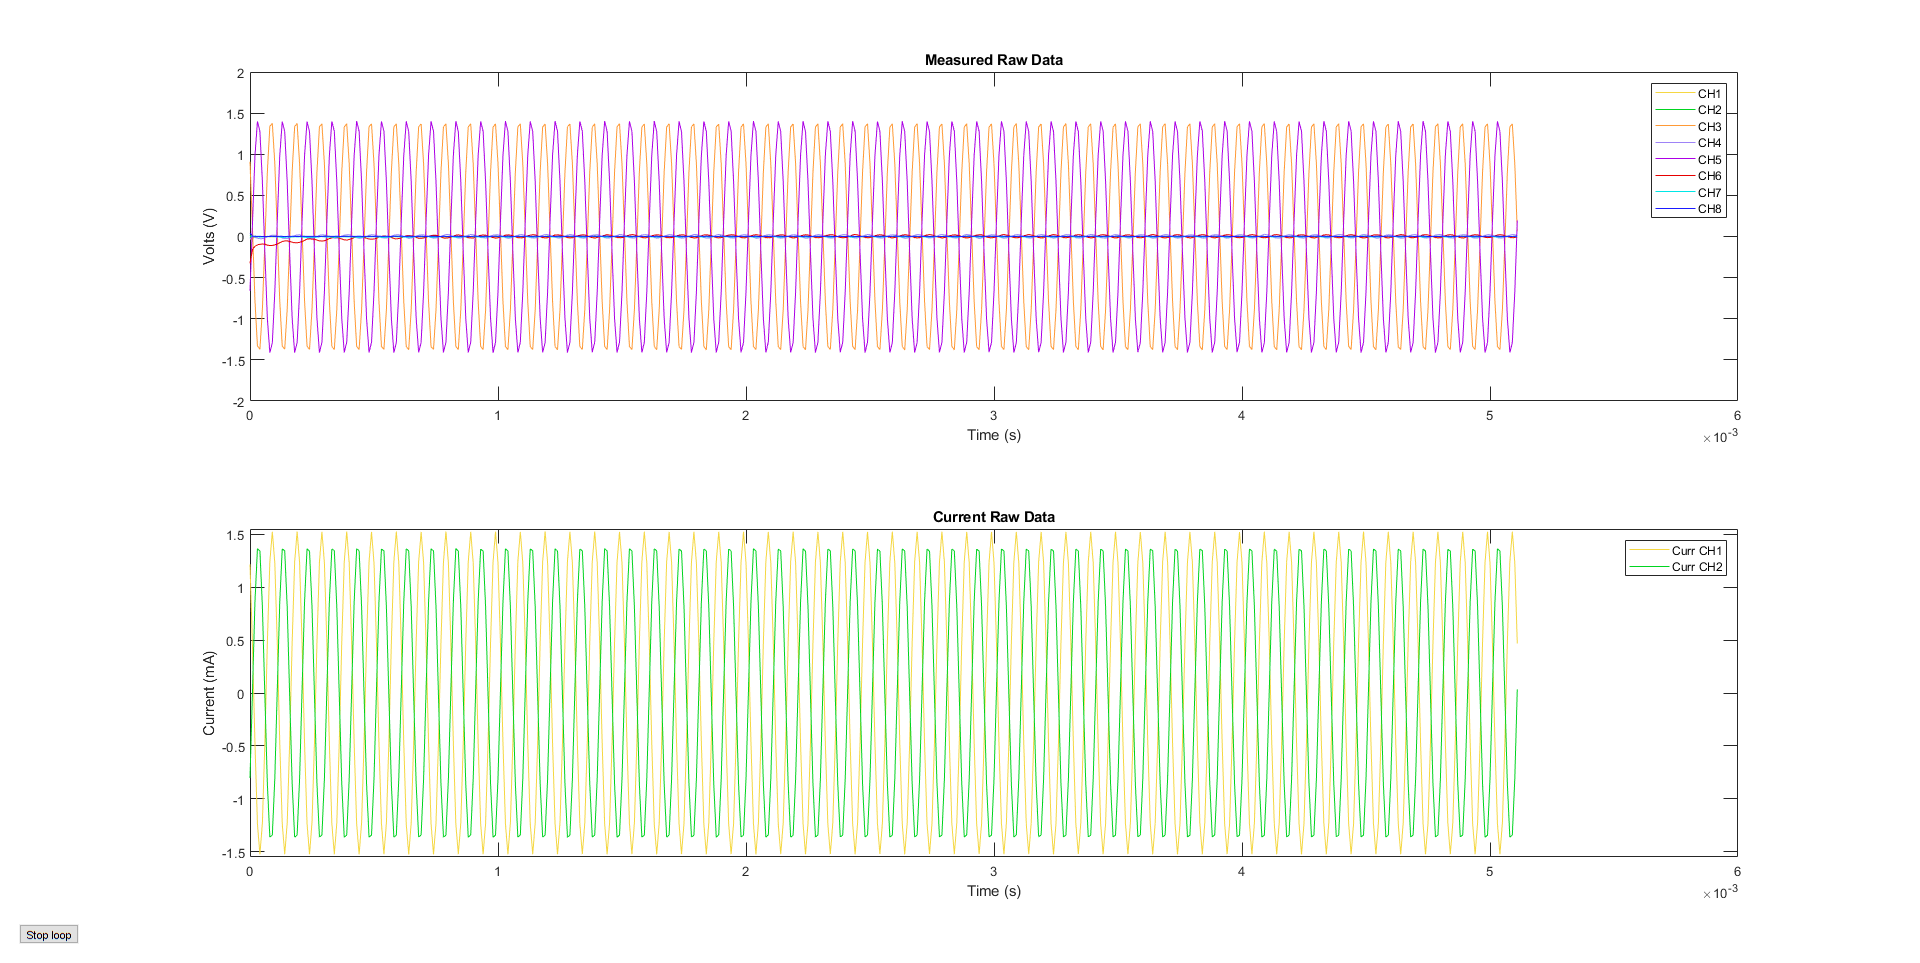
\includegraphics[width=6.5in,height=3.26181in]{media/image21.png}

Figure 4.4.3.4: Shows a plot of the voltage readings taken while testing
8 electrode channels over resistors with a 100 kilo-Ohm resistor in
series in parallel with 1kilo-Ohm resistors connecting the electrodes to
ground to simulate the grounding electrode of the testing tank

Figures 4.4.3.5 and 4.4.3.6 show voltage readings for the test set up of
an 8-electrode system connected to the saltwater testing tank. The same
characteristics of the voltage readings from this set up parallel
exactly what was observed with the 4-electrode set up. The voltage
amplitude difference between the two injection electrodes is greater
than that observed in the 4-electrode set up.

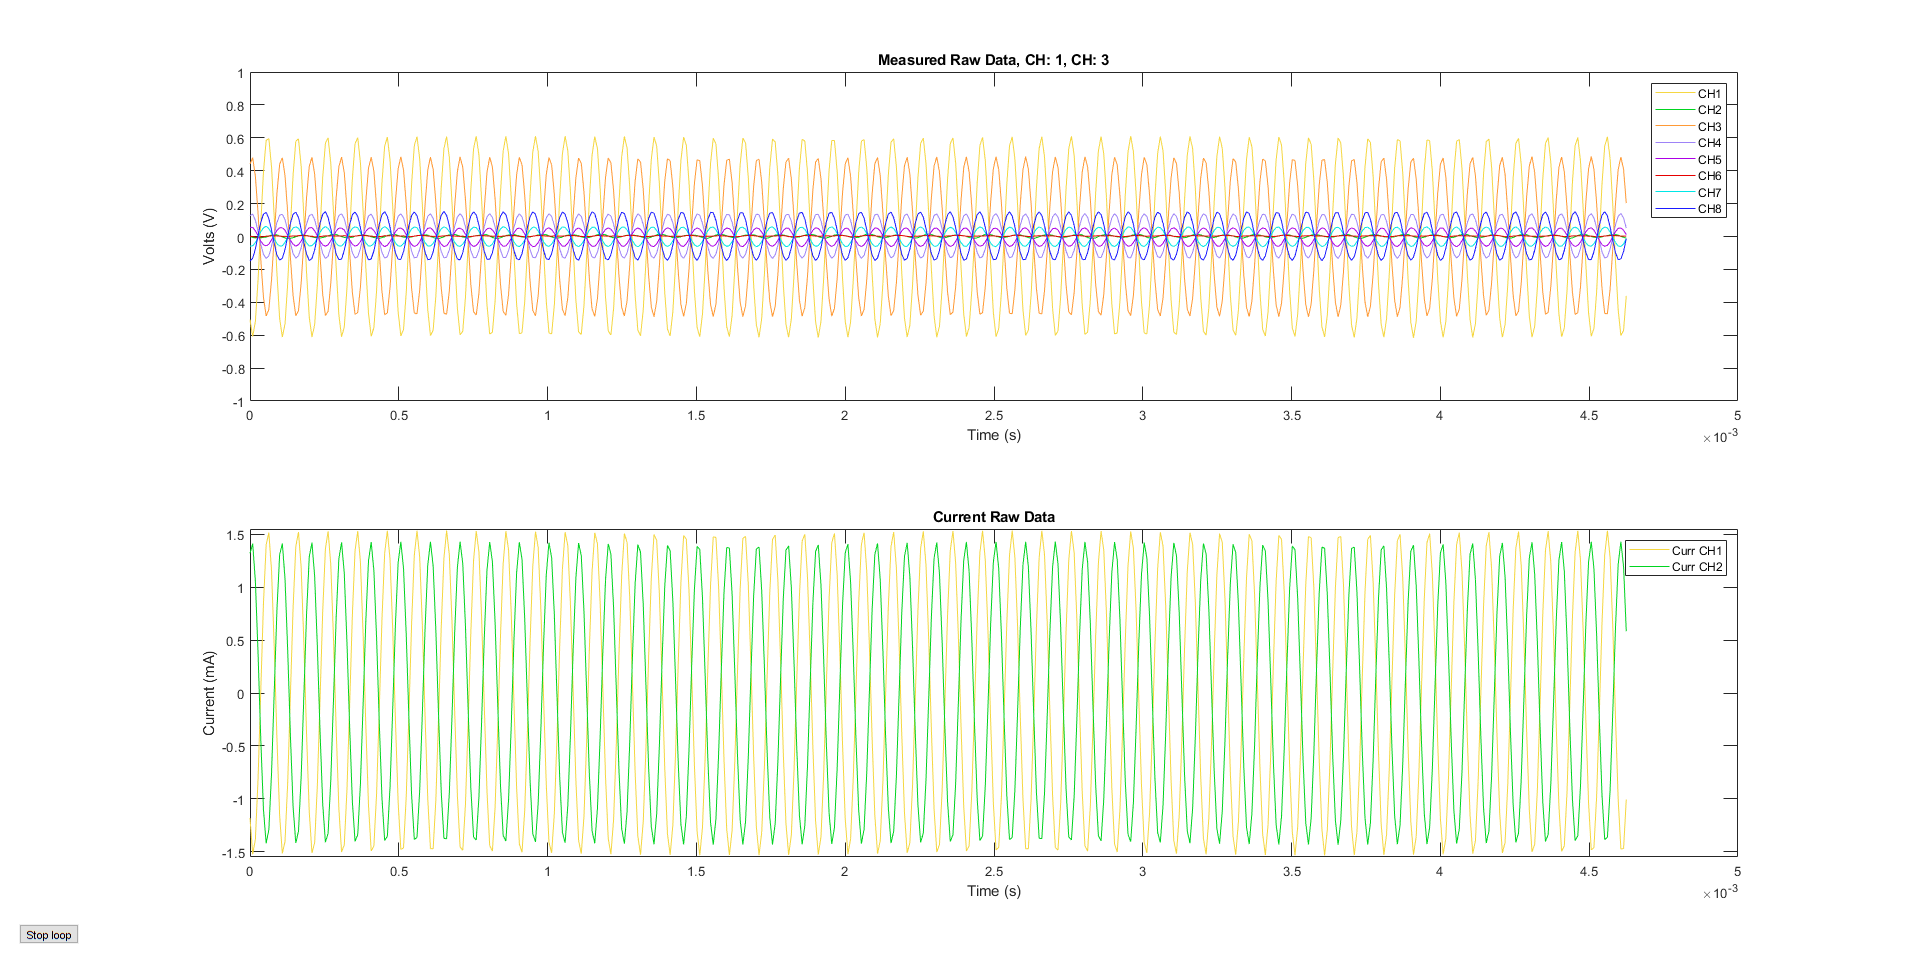
\includegraphics[width=6.5in,height=3.26181in]{media/image22.png}

Figure 4.4.3.5: Shows a plot of the voltage readings taken while testing
8 electrode channels over the testing tank with a ground connected to
the ground electrode

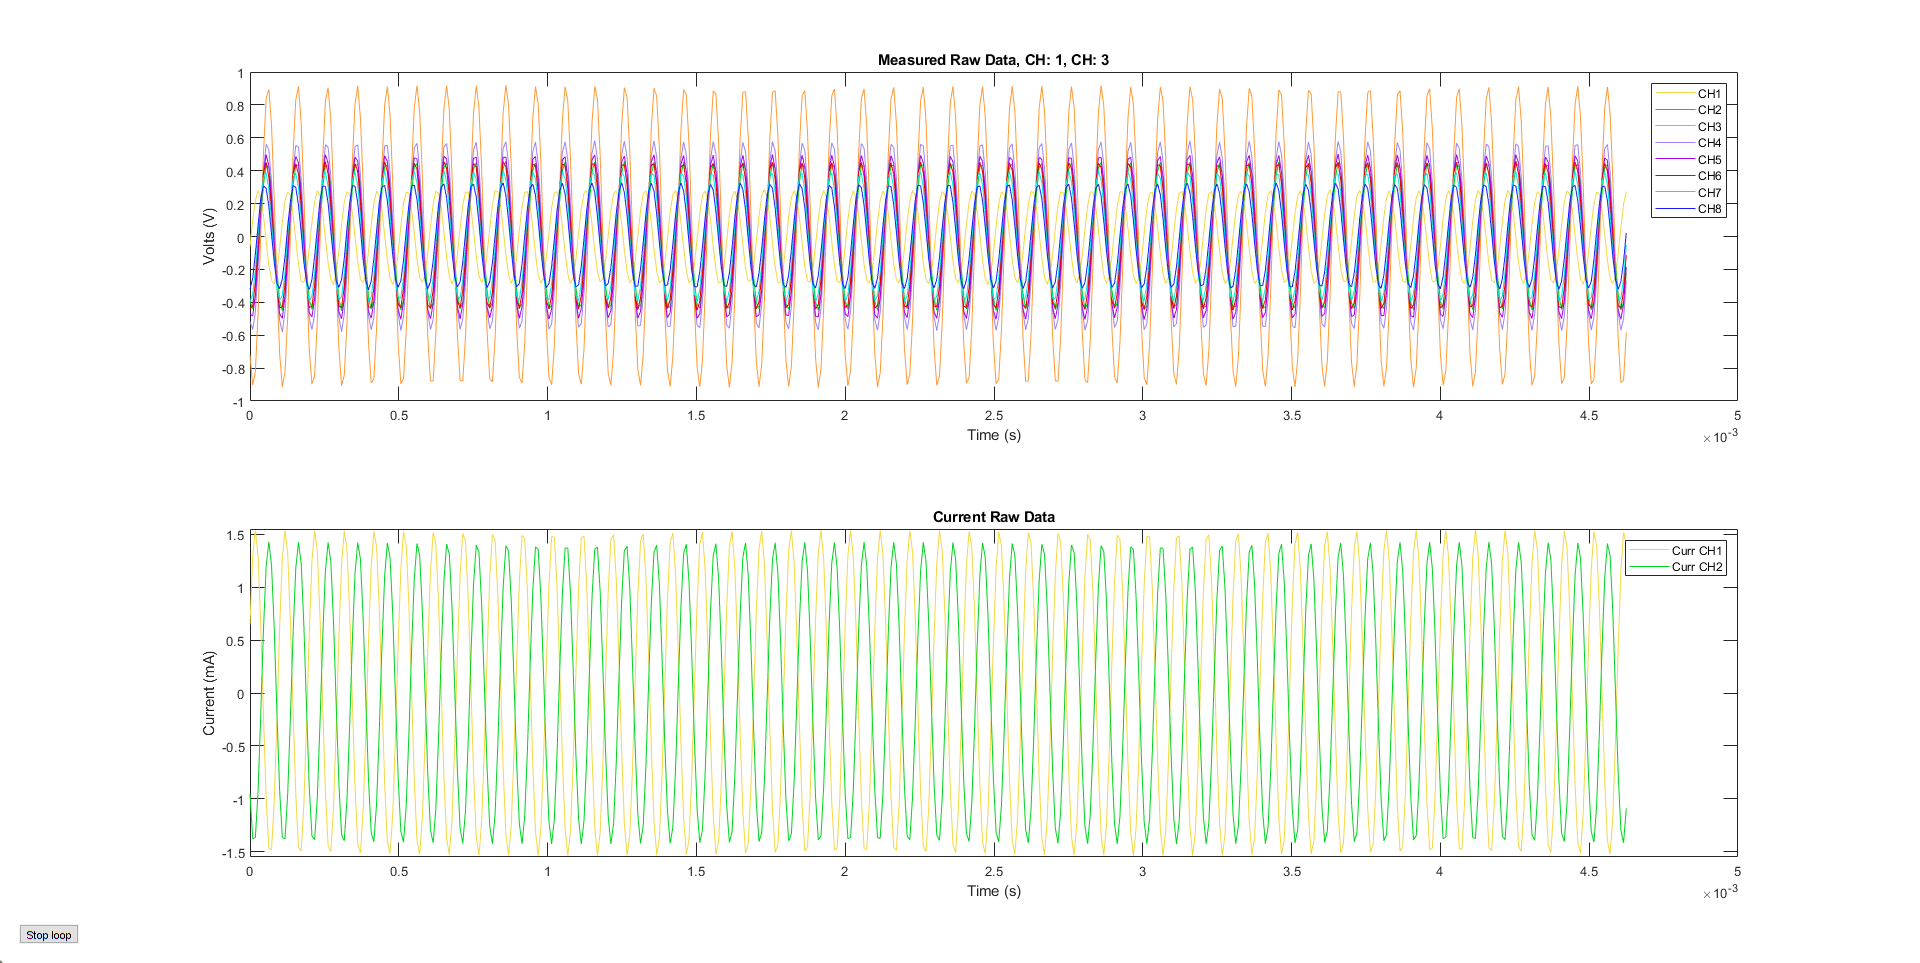
\includegraphics[width=6.5in,height=3.26181in]{media/image23.png}

Figure 4.4.3.6: Shows a plot of the voltage readings taken while testing
8 electrode channels over the testing tank without a ground connected to
the ground electrode

\subsection*{4.5 Evaluation of Data
Processing}\label{evaluation-of-data-processing}
\addcontentsline{toc}{subsection}{4.5 Evaluation of Data Processing}

\subsubsection*{\texorpdfstring{\textbf{4.5.1 Purpose of
Evaluation}~}{4.5.1 Purpose of Evaluation~}}\label{purpose-of-evaluation-3}
\addcontentsline{toc}{subsubsection}{\textbf{4.5.1 Purpose of
Evaluation}~}

Data processing was done by reading analog voltage readings from ADC
pins of the NI board. This was originally desired to be done with 32
electrodes but was reduced to 16 due to limitations of the NI board. The
sample size 1024 voltage readings were possible with the NI board and
MATLAB and simply needed to be coded in the control script. The sampling
rate of 1 Ms/s was not possible due to the NI board reducing sample rate
from the max 1 Ms/s with the addition of each ADC channel used,
resulting in 110 kS/s with 16 channels for electrodes and 2 channels for
current measurement. The voltage readings gathered in its 1024 sample by
ADC pins were then processed by the quadrature demodulation technique
explained in section 4.3. To further process the data processed by
quadrature demodulation, the results were then processed by a script
provided by Dr. Santos which cannot be explained further than that it
processes the data to produce an image, due to proprietary reasons.

\subsubsection*{\texorpdfstring{\textbf{4.5.2 Test} \textbf{Methods}
}{4.5.2 Test Methods }}\label{test-methods-3}
\addcontentsline{toc}{subsubsection}{\textbf{4.5.2 Test}
\textbf{Methods} }

\begin{itemize}
\item
  Array of data sent to QD
\item
  Then sent to image processing script
\item
  Should result in image
\item
  Will have to complete later
\end{itemize}

\subsubsection*{\texorpdfstring{\textbf{4.5.3 Results and
Discussion}~}{4.5.3 Results and Discussion~}}\label{results-and-discussion-3}
\addcontentsline{toc}{subsubsection}{\textbf{4.5.3 Results and
Discussion}~}

\begin{itemize}
\item
  To be done later
\end{itemize}

\subsection*{4.6 Evaluation of CNC Milled PCB
Process}\label{evaluation-of-cnc-milled-pcb-process}
\addcontentsline{toc}{subsection}{4.6 Evaluation of CNC Milled PCB
Process}

\subsubsection*{\texorpdfstring{\textbf{4.6.1 Purpose of
Evaluation}~}{4.6.1 Purpose of Evaluation~}}\label{purpose-of-evaluation-4}
\addcontentsline{toc}{subsubsection}{\textbf{4.6.1 Purpose of
Evaluation}~}

For the initial iteration of the EIT machine developed at the Colorado
Mesa University campus, a crucial requirement was to prototype all
circuits using CNC-milled PCBs. This was accomplished largely thanks to
the dedicated efforts of Jake Seman, a student in the electrical and
computer engineering program, whose detailed process can be found on
GitHub {[}9{]}. Jake\textquotesingle s process outlines the steps of
converting design files from KICAD, a PCB design program, into GRBR
files for milling on a CNC machine using Flatcam, and then milling on a
CNC machine using the GRBR files with the Candle program.

The objective was to evaluate whether the performance of the CNC-milled
PCBs met the specified requirements. The evaluation aimed to determine
if the milled PCBs functioned correctly according to their intended
circuit designs.

\subsubsection*{\texorpdfstring{\textbf{4.6.2 Test
Methods}}{4.6.2 Test Methods}}\label{test-methods-4}
\addcontentsline{toc}{subsubsection}{\textbf{4.6.2 Test Methods}}

To assess the quality of milled PCBs, a combination of visual inspection
and continuity checks can be employed. It is imperative that all traces
are properly isolated and connected from node to node. Initially, the
traces can be visually examined to ensure their integrity. Subsequently,
for a more objective evaluation, continuity checks are performed to
verify that the traces are routed as intended.

\subsubsection*{\texorpdfstring{\textbf{4.6.3 Results and
Discussion}~}{4.6.3 Results and Discussion~}}\label{results-and-discussion-4}
\addcontentsline{toc}{subsubsection}{\textbf{4.6.3 Results and
Discussion}~}

Initially, this process encountered numerous human errors; however, it
has since been optimized. As the group gained experience and was able to
produce a board in under an hour and achieve approximately a 2/3 success
rate in continuity testing. While this process is not as robust as
desired, it significantly expedites prototyping compared to outsourcing
the boards.

\subsection*{4.7 Conclusion and Next
Steps}\label{conclusion-and-next-steps}
\addcontentsline{toc}{subsection}{4.7 Conclusion and Next Steps}

The completion of all major components, encompassing the control system,
signal injection, and data acquisition, signifies the fulfillment of our
group\textquotesingle s proof of concept objectives. However,
it\textquotesingle s important to acknowledge that not all
specifications have been entirely met at this stage.

Particularly, the signal injection functionality employing the Howland
current source requires scrutiny to ensure a consistent current output
across the anticipated impedance range of the test subject. Moreover,
the current design involves numerous interconnecting wires linking
distinct circuits. To enhance efficiency and streamline the setup,
there\textquotesingle s an opportunity to consolidate the multiplexer
and Howland into a single circuit, thereby reducing wiring complexity.

Furthermore, while the use of single-layer, in-house milled PCBs
facilitated rapid prototyping, it limits the sophistication of the
designs. To overcome this limitation and enable the implementation of
more advanced features, it is advisable to outsource the final circuit
designs to produce more refined and technologically advanced PCBs.

The subsequent phase of data acquisition involves transitioning away
from the NI boards. Given the project\textquotesingle s open-source
nature, reliance on costly proprietary equipment should be minimized.
Instead, the next iteration would entail designing or employing more
affordable and accessible components for data collection purposes. This
approach will be the primary focus of next year\textquotesingle s
project, as it promises enhancements in sampling rate and accuracy.
Additionally, it will enable the incorporation of higher frequency
injection signals, further augmenting the system\textquotesingle s
capabilities.

The next step for enhancing the control system involves transitioning
from MATLAB to Python as an intermediate step. This transition is aimed
at facilitating a more real-time design approach. Python will play a
crucial role in improving the user interface and refining the timing of
the system, enabling the implementation of multi-threading for
simultaneous data acquisition and signal processing.

Moving away from using the NI boards is also desired. This is because
the max sample rate of ADC channels of 1 MS/s is divided by the number
of ADC channels being used, giving a max sample rate of 125 kS/s while
still being able to achieve imaging. It is recommended that further
development implements microcontrollers or FPGAs to process analog
voltage measurements into an image.

The control system is working for an 8-electrode set up. However, there
is the difference in voltage amplitude noticed for the electrodes
injecting current, as can be seen in Figure 4.3.3.2 and 4.3.2.5. This
can be corrected by increasing the input voltage signal to the smaller
amplitude signal being sent to the Howland current source.

\begin{itemize}
\item
  Need to get to 16-electrode set up
\item
  Need to get image processing done
\end{itemize}

\section*{5. Impact of Engineering
Solutions~}\label{impact-of-engineering-solutions}
\addcontentsline{toc}{section}{5. Impact of Engineering Solutions~}

The type of impact that the production of the Electrical Impedance
Tomography (EIT) machine is aimed to be an overwhelmingly positive one.
With the goal of making a relatively cheap medical imaging device even
cheaper, the team creating the EIT machine aims to help place this
technology in more hospitals and in the hands of people with little to
no funding needed. With this goal in mind, precautions need to be taken
to ensure that potential negative effects on the environment, the
economy, and society at the local and global levels are minimized.
Therefore, potential hazards are to be discussed.

\subsection*{5.1 GLOBAL IMPACTS~}\label{global-impacts}
\addcontentsline{toc}{subsection}{5.1 GLOBAL IMPACTS~}

There are positive global and local impacts that may stem from the
project\textquotesingle s main purpose of this machine, which is to
create an open-source EIT machine. This will allow the medical imaging
technique to be more widely accessible and could lead to the future of
the industry. There are limited source versions of EITs out there
because most are funded by schools and medical device companies who keep
most fundamental discoveries from research to themselves. Creation of
this open-source machine will allow the industry to have more
information as time goes on. It will lead to more designs at a cheaper
rate, help streamline the design process, allow other engineers to
reference our design, and allow others to assess both the pros and cons
of this design.

EIT is considered much safer than other common medical imaging. An EIT
machine is non-ionizing and is used for dynamic imaging. While X-rays
use electromagnetic radiation to create images of the
body\textquotesingle s internal structures. The radiation can lead to
long-term health effects like skin burns, loss of hair, and increased
incidence of cancer {[}10{]}. Magnetic Resonance Imaging (MRI) is much
safer than X-ray imaging, however the cost is very high and MRI machines
do not have much portability.

The EIT imaging process can help monitor lung function, brain activity,
and even breast cancer. It has the potential to provide real-time
imaging for various medical conditions, reducing the need for invasive
procedures and radiation exposure. With this more widely available with
the potential to increase society\textquotesingle s health. This medical
resource will be more affordable and with that, it\textquotesingle ll be
more widely used. Allowing people to understand what\textquotesingle s
happening inside their body. Published by the International
Electrotechnical Commission (IEC), the IEC 6061 is a list of technical
standards for the safety and performance of medical electrical
equipment.

\subsection*{5.2 ECONOMIC IMPACTS~}\label{economic-impacts}
\addcontentsline{toc}{subsection}{5.2 ECONOMIC IMPACTS~}

The creation of the proposed EIT machine design will have positive
economic impacts at the local and global scales. This is because the
cost for a hospital to buy most medical imaging devices is very high.
This cost is passed on to medical facility patients who can see bills in
the thousands of dollars for one round of imaging.

Magnetic Resonance Imaging (MRI) is one of the most effective and safest
imaging techniques available. They are, however, not safe to use on
anyone with implanted medical devices that consist of electrical or
metal components and is also one of the most expensive for medical
facilities to acquire. A low-end MRI machine can cost around \$150,000,
with typical costs for a device ranging from \$1 to 3 million for a
single MRI machine {[}11{]}.

X-ray imaging is less expensive but is one of the more health adverse
options for medical imaging. It is also one of the less versatile as its
main use is on the imaging of bones. Portable x-ray devices may range
from \$5 to \$60 thousand dollars. Portable devices are less versatile
than their stationary counterparts commonly found in hospitals, which
are necessary for general and emergency care use. Stationary x-ray
machines can range from \$35,000 to \$200,000 {[}12{]}.

Ultrasound devices are considered the safest classical medical imaging
devices, and one of the cheapest. They do have limitations though, as
they cannot penetrate bone, air filled cavities, and cannot penetrate
deep into the body {[}13{]}. Low end devices may cost from \$5,000 to
\$10,000. Mid-grade to high end ultrasound devices cost from \$20,000 to
\$200,000.

As EIT is one of the youngest medical imaging technologies, it is also
one of the least developed. From directly messaging the medical device
company Dräger, the team received a quote of \$60,000 dollars for their
device. This is far above what the team believes an open-source EIT
machine could cost, with high quality imaging. Using relatively
inexpensive components, the team estimates that construction of an EIT
machine could cost no more than a few thousand dollars at most.

If such cheap medical imaging devices for heart, lungs, brain, and
breast cancer were available, it could drastically reduce the cost for
hospitals to view these parts of the body. These savings would be past
on to patients. Therefore, a relatively cheap, open source EIT machine
would have an overwhelmingly positive economic impact.

\subsection*{5.3 ENVIRONMENTAL IMPACTS~}\label{environmental-impacts}
\addcontentsline{toc}{subsection}{5.3 ENVIRONMENTAL IMPACTS~}

EIT devices may contain materials such as heavy metals and toxic
materials, as all electronic components do, especially when it comes to
printed circuit boards (PCBs). This type of waste material is commonly
called e-waste. E-waste can contain substances such as lead, mercury,
and other metals, flame retardants, and certain phthalates {[}14{]}.
This weighs into the economic and environmental impacts because most
local ordinances require an individual or business to pay to have
e-waste properly disposed of. In the case of the design presented in
this paper, PCBs will be constructed, wires will connect PCBs and
components, and some wire connected electrodes will have been used.
Therefore, the only 2 precautions needed are to properly recycle e-waste
upon disposal of the EIT machine, or its components, at places like
local landfills.

While the disposal of e-waste can have negative effects on the
environment, the manufacturing process involves the extraction of raw
materials, energy consumption, and transportation, all of which have
environmental consequences {[}{[}15{]}. Fossil fuels are used to mine
raw materials and fossil fuels are also used to transport raw materials
and manufactured components. Although extraction and transportation of
raw materials is argued to negatively impact the environment, it is
impossible to get the components required for an EIT machine without
these effects. It is currently widely considered more important to have
access to electronic components than it is to avoid any possible
negatives.

\subsection*{5.4 SOCIETAL IMPACTS~}\label{societal-impacts}
\addcontentsline{toc}{subsection}{5.4 SOCIETAL IMPACTS~}

There are possible humanitarian concerns when it comes to conditions for
workers in fabrication facilities related to the production of
electronic components. In China for example, Apple device manufacturing
facilities have worker conditions documented which many would call cruel
and border basically slavery. Cheap labor and lax environmental
regulations have led to concerns about worker rights and pollution
{[}16{]}. This is not the case for all electronic component factories.
And there are no known or reasonably suggestable reasons for concerns
about humanitarian issues from any electronic component manufacturer
that is involved in the production of any electronic component or PCB in
the current design plan for the EIT machine.

When considering potential environmental, economic, global, and local
costs to the potential benefit of the EIT machine design and its
implementation, the benefits far outweigh the costs. Environmental
negative impacts are small. Positive economic, global, and local impacts
are potentially extremely positive. Medical bills for imaging certain
parts of the human body can be severely reduced. EIT imaging could even
be brought to remote parts of the world without power grids, given a
sufficient and stable power source. EIT has the potential to be designed
by hobbyists and those with the need for it, safely, in their own homes.
Overall, EIT will have a positive impact on the world and has the
potential to improve the health of people around the world.

\section*{}\label{section}
\addcontentsline{toc}{section}{}

\section*{5. References~}\label{references}
\addcontentsline{toc}{section}{5. References~}

{[}1{]} ``Electrical impedance tomography,'' \emph{Wikipedia}. Sep. 17,
2023. Accessed: Oct. 19, 2023. {[}Online{]}. Available:
https://en.wikipedia.org/w/index.php?title=Electrical\_impedance\_tomography\&oldid=1175791739

{[}2{]} S. Mansouri, Y. Alharbi, F. Haddad, S. Chabcoub, A. Alshrouf,
and A. A. Abd-Elghany, ``Electrical Impedance Tomography -- Recent
Applications and Developments,'' \emph{J Electr Bioimpedance}, vol. 12,
no. 1, pp. 50--62, Nov. 2021, doi: 10.2478/joeb-2021-0007.

{[}3{]} ``Talles Santos \textbar{} Colorado Mesa University.'' Accessed:
Oct. 27, 2023. {[}Online{]}. Available:
https://www.coloradomesa.edu/directory/computer-science-engineering/talles-santos.html

{[}4{]} ``Electrical Impedance Tomography (EIT) Device - LuMonTM,''
Sentec. Accessed: Nov. 14, 2023. {[}Online{]}. Available:
https://www.sentec.com/electrical-impedance-tomography/

{[}5{]} ``Electrical Impedance Tomography \textbar{} Draeger.''
Accessed: Nov. 14, 2023. {[}Online{]}. Available:
https://www.draeger.com/en\_uk/Hospital/Electrical-Impedance-Tomography

{[}6{]} ``Sciospec's EIT Electrical Impedance Tomography - Sciospec.''
Accessed: Nov. 14, 2023. {[}Online{]}. Available:
https://www.sciospec.com/eit/

{[}7{]} ``IEC 60601,'' \emph{Wikipedia}. Apr. 08, 2023. Accessed: Nov.
14, 2023. {[}Online{]}. Available:
https://en.wikipedia.org/w/index.php?title=IEC\_60601\&oldid=1148739103

{[}8{]} ``ANSI/AAMI ES60601-1:2005/Amendments - Medical electrical
equipment --- Part 1: General requirements for basic safety and
essential performance, Amendments.'' Accessed: Nov. 14, 2023.
{[}Online{]}. Available:
https://webstore.ansi.org/standards/aami/ansiaamies606012005amendments

{[}9{]} J. Seman, ``Jbsco/PCB\_MFG.'' Mar. 21, 2024. Accessed: Apr. 09,
2024. {[}Online{]}. Available: https://github.com/Jbsco/PCB\_MFG

{[}10{]} ``Risks of Radiation,'' UCSF Radiology. Accessed: Oct. 27,
2023. {[}Online{]}. Available:
https://radiology.ucsf.edu/patient-care/patient-safety/radiation-safety/risks-of-radiation

{[}11{]} ``Why Are MRIs So Expensive at Hospitals?,'' Heartland Imaging.
Accessed: Oct. 27, 2023. {[}Online{]}. Available:
https://heartlandimagingcenters.com/2021/03/19/why-are-mris-so-expensive-at-hospitals/

{[}12{]} C. Hutchison, ``What Is the Average Cost of an X-Ray Machine?
{[}Updated 2023{]}.'' Accessed: Oct. 27, 2023. {[}Online{]}. Available:
https://www.mavenimaging.com/blog/average-x-ray-machine-cost

{[}13{]} ``Ultrasound - Mayo Clinic.'' Accessed: Oct. 27, 2023.
{[}Online{]}. Available:
https://www.mayoclinic.org/tests-procedures/ultrasound/about/pac-20395177

{[}14{]} K. K. Kefeni, J. O. Okonkwo, O. I. Olukunle, and B. M. Botha,
``Brominated flame retardants: sources, distribution, exposure pathways,
and toxicity,'' \emph{Environ. Rev.}, vol. 19, no. NA, Art. no. NA, Dec.
2011, doi: 10.1139/a11-010.

{[}15{]} ``Natural-Resource Use and Environmental Impacts \textbar{} One
Planet network.'' Accessed: Oct. 27, 2023. {[}Online{]}. Available:
https://www.oneplanetnetwork.org/SDG-12/natural-resource-use-environmental-impacts

{[}16{]} ``How the iPhone Helps Perpetuate Modern-Day Slavery,''
HuffPost. Accessed: Oct. 27, 2023. {[}Online{]}. Available:
https://www.huffpost.com/entry/how-the-iphone\_b\_5800262

~

\section*{6. Appendices~}\label{appendices}
\addcontentsline{toc}{section}{6. Appendices~}

\textbf{A:}

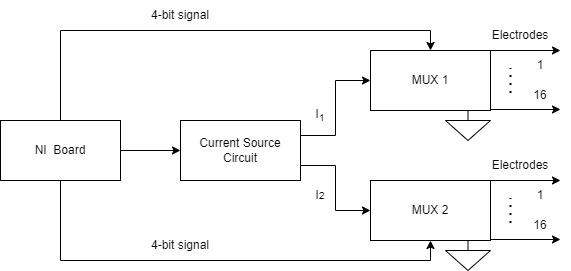
\includegraphics[width=5in,height=2.375in]{media/image24.jpg}

\end{document}